\documentclass[10pt]{article}

\usepackage[preprint]{tmlr}
\usepackage[T1]{fontenc}
\usepackage{lmodern}
\usepackage{amsmath,amssymb,amsthm,mathtools}
\usepackage{array}
\usepackage{natbib}
\usepackage{microtype}
\usepackage{hyperref}
\usepackage{booktabs}
\usepackage{enumitem}
\usepackage{graphicx}
\usepackage{tikz}
\usetikzlibrary{arrows.meta,positioning}
\usepackage{placeins}
\usepackage{algorithm}
\usepackage{algpseudocode}

\hypersetup{colorlinks=true,allcolors=blue,hypertexnames=false}
\emergencystretch=3em

% Keep figures at the top when LaTeX places them on a float-only page.
\makeatletter
\setlength{\@fptop}{0pt}
\makeatother

\newtheorem{proposition}{Proposition}
\newtheorem{lemma}{Lemma}
\newtheorem{theorem}{Theorem}
\newtheorem{corollary}{Corollary}
\theoremstyle{definition}
\newtheorem{definition}{Definition}
\newtheorem{remark}{Remark}
\newtheorem{assumption}{Assumption}

\DeclareMathOperator{\NF}{NF}
\newcommand{\Lie}{\mathcal{L}}
\newcommand{\Eref}{E_{\mathrm{ref}}}

% Fit wide tables to the text block without enlarging narrower tables.
\newsavebox{\tablebox}
\newcommand{\fittable}[2][\linewidth]{%
  \sbox{\tablebox}{#2}%
  \ifdim\wd\tablebox>#1\relax
    \resizebox{#1}{!}{\usebox{\tablebox}}%
  \else
    \usebox{\tablebox}%
  \fi}

\title{Diagnosing Model and Discretisation Errors in Reinforcement Learning Simulators Using Invariants}
\author{Tesfay Zemuy Gebrekidan\\
  Independent Researcher}
\date{}

\begin{document}
\maketitle
\begingroup
\renewcommand{\thefootnote}{}
\footnotetext{OpenAI's Codex was used to assist with manuscript editing,
code changes and consistency checks. The author is responsible for the
claims and results.}
\endgroup

\begin{abstract}
Energy drift in a reinforcement-learning simulator can arise from incorrect
dynamics or discretisation error. We distinguish these using a specified
invariant, double-precision (float64) state and a callable step map, without
requiring trajectories from a trusted, fault-free simulator. An exact
layer tests symbolic invariance through Lie derivatives and ideal membership.
A numerical layer re-integrates each step at four refinement levels and
measures how its energy defect decays. Under smoothness and nondegeneracy
conditions, the refinement exponents approach the achieved integrator order
for conserving dynamics and zero for a nonzero invariant-breaking rate. A
numerical classifier uses this refinement pattern and abstains when round-off or noise
dominates. On Gymnasium Acrobot, it labels $1000/1000$ healthy starts consistent;
in a separate held-out test, $2/40$ healthy starts using fourth-order
Runge--Kutta integration at a timestep of $0.2$ seconds receive
the fallback label order-4 rather than consistent. It detects parameter errors
in $\ge86.7\%$ of starts at $10^{-5}$; detection is partial at $10^{-6}$ ($1/30$--$14/30$). With the same constants,
it raises no fault flags across $1440$ healthy evaluations of $120$ starts on
three further systems, with $90.3\%$ coverage. Audits expose stale-parameter
inconsistencies in CartPole and second-order trajectory convergence in
conservative Ant and Humanoid models in MuJoCo 3.16.0 despite selection of
fourth-order Runge--Kutta integration;
a separately tested MuJoCo development revision incorporating a
Runge--Kutta--Munthe-Kaas correction to rotational integration exhibits
fourth-order trajectory convergence in the same models. Controlled tests
and a conditional Magnus derivation link the order loss to the orientation update;
a commutator-free update restores fourth order in a heavy-top replica. The
method supplies fault-class information without improving detection floors
over a matched-step reference-based screen; cancellation of error terms at nonzero timesteps and
masked model errors remain limitations.
\end{abstract}

\section{Introduction}

A reinforcement-learning (RL) simulator defines the transitions from which an
agent learns. If its implemented dynamics differ from the intended system,
training can succeed on the wrong task. Dynamics randomisation is used to
reduce simulation-to-reality mismatch by varying physical parameters during
training \citep{peng2018}. Each assignment must remain consistent with the
executed dynamics. A changed mass attribute may leave a cached constant
unchanged, while a selected integrator may fail to achieve its declared order
for a particular state representation. These cases require different remedies:
correcting the equations or parameter updates in the first case, and
inspecting the numerical update in the second. Energy drift alone does not
tell them apart, since a conserving model can also drift under discretisation.

Our audits illustrate both problems: parameter updates in Gymnasium CartPole
can leave cached dynamics inconsistent with the declared parameters, while
conservative Ant and Humanoid models in MuJoCo 3.16.0 exhibit second-order
trajectory convergence despite selection of fourth-order Runge--Kutta
integration (RK4). The latter finding concerns the tested version and setup;
a separately tested development revision exhibits fourth-order convergence.

\paragraph{Motivation.}
Reference-based invariant screening can identify a broken physical constraint
and attribute it to a parameter \citep{gebrekidan2026diagnosing}.
A healthy reference may be unavailable for a shipped environment; even when one
exists at nominal parameters, it is not a matched reference for every new
randomised instance. An energy law can still be available from the declared
parameters or the engine itself. State self-convergence estimates numerical
order without an exact solution \citep{roache1998,nparcconvergence}, but RK4
can converge at fourth order while discretising incorrect equations. We ask
whether a specified invariant and access to the step map can distinguish
invariant-breaking dynamics from discretisation error without a healthy run
or a fitted healthy-drift threshold.

On Acrobot, \citet{gebrekidan2026diagnosing} report that, at its shipped step
$\Delta t=0.2$, RK4 energy drift exceeds the effect of a $1\%$ parameter error;
their sensitivity sweeps use $\Delta t=0.005$. We retain the deployed macro-step
as the diagnostic interval and re-integrate it at $m=1,2,4,8$ sub-steps. This
measures how the defect decays under refinement and requires calls at finer
steps, beyond native-step logs.

\paragraph{Approach and contributions.}
We assume a specified invariant, readable double-precision floating-point
(float64) internal state, a known declared integrator order, and a step map
that can be restarted from the same state at different timestep sizes.
The numerical tests concern passive, smooth conservative dynamics.
We call the pattern of energy defects across timestep refinements the
\emph{energy fingerprint}. The diagnostic classifies this pattern and
abstains when the signal is unresolved. When symbolic equations are also
available, an optional exact test checks whether those equations preserve
the specified invariant. Our contributions are:
\begin{enumerate}[label=(\alph*)]
  \item \textbf{Symbolic test.} We state the Lie-derivative criterion for
  polynomial and denominator-cleared rational fields
  (Proposition~\ref{prop:invariance}) and compute a 14-term Acrobot fault
  signature (\S\ref{sec:acrobot-cert}).
  \item \textbf{Numerical diagnosis.} We derive the refinement-order signal
  (Theorem~\ref{thm:fp}) and give a finite-step classifier with abstention
  (Algorithm~\ref{alg:classifier}). Validation covers shipped Acrobot,
  integrators of orders $1$--$4$, three further systems with unchanged
  classifier constants, and threshold sensitivity
  (\S\ref{sec:validation}, \S\ref{sec:robustness}).
  \item \textbf{Simulator audits.} We test parameter consistency in Gymnasium
  and declared integrator order in eleven MuJoCo environments
  (\S\ref{sec:audits}). Controlled quaternion models, a conditional Magnus
  derivation, an independent replica and a source build with a
  Runge--Kutta--Munthe-Kaas (RKMK) correction explain
  the observed order loss and recovery (\S\ref{sec:audit:quat}). A regime gate
  extends the test to sampled constraint-free steps (Appendix~\ref{sec:audit:gate}).
  \item \textbf{Comparisons.} Matched-step reference screening, direct
  reference-step comparison and same-call state self-convergence establish
  the diagnostic's sensitivity and fault-class information
  (\S\ref{sec:position}). Order-adapted extrapolation helps on the tested
  low-order integrator (Appendix~\ref{app:extrap}).
\end{enumerate}

The symbolic test establishes whether the specified equations preserve the
invariant; it does not certify the simulator implementation. The numerical
diagnostic returns \emph{consistent}, \emph{model} or \emph{order-$k$}, or
abstains. These finite-step classifications are heuristic: the convergence
theorem is asymptotic and does not guarantee individual labels. An invariant
gives a partial physical specification, so changes that preserve it remain
undetected. Classifier constants were set during Acrobot development; guards
depend on units and an optional supplied noise level.

\section{Related work}\label{sec:related}

We review symbolic invariance tests, reference-based diagnosis and numerical
refinement methods, together with geometric integration and noisy residuals.
These approaches differ in what they reveal about model and numerical error.

\paragraph{Symbolic invariance and reference-based diagnosis.}
Symbolic invariance tests check whether specified equations preserve a
constraint. Lie-derivative tests are established for polynomial equalities
\citep{ghorbal2014}, while differential-elimination methods such as
$\mathrm{RGA}_o$ generate and check invariant sets for polynomial ODEs
\citep{simmons2026}. Barrier certificates address the related problem of
safety verification \citep{prajna2004}. These methods check supplied equations; a simulator can still depart from them. To diagnose such discrepancies, \citet{gebrekidan2026diagnosing}
compare candidate and healthy simulator logs using canonical polynomial
invariants, localise broken constraints and attribute faults to parameters.
However, this comparison requires a matched healthy reference. Our numerical
test assumes a specified conserved quantity and does not require healthy
logs; invariant recovery, constraint localisation and general parameter
attribution are outside its scope. Invariant discovery could supply
candidates for this test, provided they are certified against the nominal
model and frozen before testing. This interface is not implemented here.
Moreover, an invariant set need not define a smooth scalar conserved quantity
on an open neighbourhood, as required by the energy fingerprint.

\paragraph{Energy drift in learned and simulated dynamics.}
Energy drift measures departures from conservation along a trajectory.
For example, \citet{xiao2026lawm} evaluate a
variational-integrator world model using relative energy drift and a discrete
Euler--Lagrange residual. Similarly, \citet[\S5.1 and Appendix~D.1]{yuan2026newtongen} use a Physical
Invariance Score, adapted from prior work, based on the temporal mean and
standard deviation of a quantity that should remain invariant. However, both model and numerical error contribute to these measurements,
so raw drift alone does not distinguish them. Our test requires a callable step map at refined timesteps, which a learned
transition trained at one frame interval generally does not provide.

\paragraph{State self-convergence and defect extrapolation.}
Step-refinement studies are standard tools for code verification
\citep{roache1998,oberkampf2010}. State self-convergence estimates numerical
order by comparing solutions computed at successively smaller timesteps,
without requiring an exact solution \citep{nparcconvergence}. However, an
integrator can retain its declared order while solving incorrect equations.
The model error shared by the refined runs cancels in their state
differences. Checking a solver against a manufactured solution or a conserved
quantity provides another verification route \citep{salari2000}, although
manufactured solutions require a known test problem and control of its
equations or forcing.

Richardson extrapolation removes a leading discretisation term using an
assumed error expansion \citep{richardson1927}. Applied to invariant defects,
it can estimate the component that persists under refinement. We call this
measurement \emph{defect extrapolation}. Remainder terms and noise still
affect the estimate, and a threshold on its magnitude does not by itself
identify a fault class. Our energy fingerprint instead uses the refinement
pattern to distinguish invariant-breaking dynamics from resolved numerical
error, with abstention when the signal is insufficient. Modified-equation
analysis supplies our defect expansion \citep{hairer2006geometric}.
Section~\ref{sec:selfconv} compares the fingerprint and state self-convergence
using identical simulator calls.

\paragraph{Geometric integration.}
Variational and symplectic integrators preserve geometric structure and can
have favourable long-time energy behaviour
\citep{marsden2001,hairer2006geometric}. However, they do not generally
conserve the original energy exactly. Lie-group Runge--Kutta methods are
designed to retain their order on manifolds
\citep{crouch1993,munthekaas1998,celledoni2003}, and the Magnus expansion
provides a standard tool for analysing the exponent \citep{blanes2009}.
Basilisk documents the second-order limitation of a single-exponential
attitude update and a stage-wise quaternion alternative
\citep{basiliskmjscene}. Our MuJoCo audit builds on this context by testing
benchmark models and examining when orientation error appears in energy
(\S\ref{sec:audit:quat}). The fingerprint can also be used with geometric
integrators if the energy defect has a nonzero leading coefficient. Exact
energy preservation removes this signal (Remark~\ref{rem:conserving}).

\paragraph{Noisy residuals and refinement data.}
Numerical integration can also affect residuals used for fault diagnosis.
\citet{mohammadi2023} study this effect in neural-ODE residual models for a
truck after-treatment system. Our tests use known invariants and a callable
simulator step map. For noisy refinement data, \citet{oliver2014} combine
sampling-error estimation, including temporal correlation, with Bayesian
Richardson extrapolation to estimate uncertainty in simulation statistics.
Applying that approach to our measurements would require a likelihood for
the shared-start, absolute residuals and a choice of priors. This comparison
remains open. We instead derive the noise gain of defect extrapolation in
Appendix~\ref{app:extrap} and test the fingerprint's noise guard in
\S\ref{sec:exp:noise}.

These approaches leave a diagnostic gap when no healthy reference is
available: symbolic tests check equations, raw drift combines error sources,
and self-convergence measures candidate order. Our energy fingerprint uses the
refinement pattern of a specified energy defect to distinguish
invariant-breaking dynamics from numerical error. It provides a heuristic
model/order label rather than a general correctness certificate: cancellation,
masking and invariant-preserving faults remain limitations.
Table~\ref{tab:capabilities} summarises the information requirements,
conclusions and limitations of the five diagnostics discussed above and our
energy fingerprint.

\begin{table}[htbp]
\centering\small
\begin{tabular}{>{\raggedright\arraybackslash}p{3.1cm}>{\raggedright\arraybackslash}p{4.6cm}>{\raggedright\arraybackslash}p{6.4cm}}
\toprule
Diagnostic & Required information & Conclusion and main limit \\
\midrule
Symbolic invariance & field, invariant, algebraic constraints & exact test of the specified model; not its implementation \\
Reference screening & invariants, healthy/candidate logs & discrepancy, localisation and parameter attribution; needs a matched reference \\
Raw energy drift & invariant, candidate trajectory & departure from conservation; pools model and numerical error \\
State self-convergence & restartable refined step map & achieved state order; wrong equations can retain the declared order \\
Defect extrapolation & invariant, refined step map, assumed order & persistent-defect estimate; remainders and noise remain; no fault class from a scalar threshold \\
Energy fingerprint (this work) & invariant, refined step map, float64 state, declared order & heuristic model/order label with abstention; cancellation, masking and invariant-preserving faults remain \\
\bottomrule
\end{tabular}
\caption{Information requirements and conclusions of the diagnostics.
Self-convergence and the fingerprint need no healthy-run threshold calibration;
the fingerprint uses development-set constants. Extrapolation also needs no
healthy run to compute its statistic; the thresholded comparator in
Table~\ref{tab:extrap-main} uses healthy-run calibration.}
\label{tab:capabilities}
\end{table}

\section{Method}\label{sec:method}

\subsection{Problem and access model}\label{sec:setting}

The reference system is $\dot x=f_0(x,u)$ with state $x\in\mathbb R^n$ and
parameters $\theta$. A \emph{candidate} implementation is a one-step map
$\Psi_\tau(x,u)$. Constraints $h_i(x)=0$ define a real algebraic set $V$
with \emph{real vanishing ideal}
$I(V)=\{p\in\mathbb R[x]: p|_V=0\}$, which can be strictly larger than the
ideal generated by the $h_i$.

\begin{assumption}[Access]\label{ass:access}
(A1) $\Psi_\tau$ can be evaluated at arbitrary $\tau$ from an arbitrary
state in floating point, and the internal state (not only a
lower-precision observation) is readable. (A2) A reference invariant $E$
with $\Lie_{f_0}E=0$ can be \emph{evaluated}, not necessarily written in
closed form: the refinement layer uses only smoothness of $E$. (A3) The
declared integrator order $q$ is known (for Gymnasium's \texttt{rk4}, $q=4$;
for CartPole's Euler, $q=1$).
\end{assumption}

The invariant specifies the parameters against which the simulator is tested.
In the CartPole audit these are the simulator's own declared parameters; in
MuJoCo the engine evaluates the energy through \texttt{mj\_energy}. The exact
layer requires a polynomial $E$, as obtained for Acrobot and CartPole by
lifting $\cos\theta,\sin\theta$ to variables. Invariant recovery is outside
this study (\S\ref{sec:related}).

Assumption (A1) holds for
Gymnasium's \texttt{AcrobotEnv} and \texttt{CartPoleEnv}, whose step-size
attribute is writable and whose state is float64. It does not hold for a
compiled black box with a fixed step or float32-only observations. The
reference-based screen instead uses logged states from healthy and candidate
runs (Table~\ref{tab:capabilities}).

\subsection{Diagnostic workflow}\label{sec:workflow}

Freeze the invariant, nominal parameters and energy units. Optionally check
symbolic invariance (\S\ref{sec:exact}), then restore each sampled state and
re-integrate the same interval $h$ at $m=1,2,4,8$ sub-steps. Average the
absolute endpoint energy defects and apply Algorithm~\ref{alg:classifier}
($15$ simulator steps per state). Numerical labels are heuristic; follow-up
checks are given in \S\ref{sec:deployment}.

\subsection{Optional exact invariance test}\label{sec:exact}

This optional layer checks symbolic equations; the numerical diagnostic can be
used independently.

For differentiable $p$ and field $f$, $\Lie_fp=\nabla p^\top f$ and
$\frac{d}{dt}p(x(t))=\Lie_fp(x(t))$ along solutions.

Equality-invariance criteria based on Lie derivatives are established in
\citet{ghorbal2014}. We express the criterion as polynomial ideal membership
and use Gr\"obner-basis reduction to compute it. For a fixed monomial order,
a Gr\"obner basis $G$ of an ideal $I$ allows any polynomial $p$ to be reduced
to a unique normal form, denoted $\NF_G(p)$; this normal form is zero if and
only if $p\in I$ \citep{cox2015}. We state the resulting invariance test below.

\begin{proposition}[Invariance criterion]\label{prop:invariance}
Let $f$ be a polynomial vector field, let
$V$ be a real algebraic set, and let $p_1,\dots,p_r$ generate $I(V)$. Then
$V$ is invariant under the flow of $f$ if and only if
\begin{equation}\label{eq:lie-ideal}
  \Lie_f p_i\in I(V),\qquad i=1,\dots,r.
\end{equation}
Consequently, if $G$ is a Gr\"obner basis of $I(V)$, the criterion can be
checked by the finite set of reductions $\NF_G(\Lie_fp_i)=0$,
$i=1,\dots,r$.
\end{proposition}

\begin{proof}
($\Rightarrow$) For $x\in V$ and $p\in I(V)$, invariance gives
$p(x(t))=0$ near $0$; differentiating at $t=0$ gives $\Lie_fp(x)=0$, so
$\Lie_fp\in I(V)$.
($\Leftarrow$) By the Leibniz rule
$\Lie_f(\sum a_ip_i)=\sum(\Lie_fa_i)p_i+a_i\Lie_fp_i\in I(V)$, hence
$\Lie_f^kp_i\in I(V)$ for all $k$. For $x\in V$ the real-analytic function
$t\mapsto p_i(x(t))$ has all derivatives at $0$ equal to
$\Lie_f^kp_i(x)=0$, so it vanishes near $0$; thus $x(t)\in V$ near $0$. The
set of times with $x(t)\in V$ is closed in the maximal interval, and open by
the same argument at any such time, hence is the whole interval.
\end{proof}

\begin{remark}[Scope of the criterion]
Polynomial fields are analytic, as used in the sufficiency proof. For an
arbitrary real-analytic field, $\Lie_fp$ need not be polynomial, so the
polynomial ideal-membership and Gr\"obner-reduction test above does not
directly apply. A positive result certifies the \emph{specified symbolic
model}, not a floating-point implementation. Mass-matrix inverses make
mechanical fields rational with denominator $\delta>0$; the polynomial field
$\tilde f=\delta f$ has the same orbits, the same invariant sets, and
$\Lie_{\tilde f}p=\delta\Lie_fp$, so the proposition applies to $\tilde f$.
\end{remark}

For a candidate with consistent field $f_j$ the \emph{algebraic signature}
is $\sigma_{\mathrm{alg}}(F_j)=(\NF_G(\Lie_{f_j}p_i))_i$; a zero entry means
that infinitesimal test passes, and an all-zero signature does not show
$f_j=f_0$. For example, $h=x^2+y^2-1$ and $f_\epsilon=(-y,(1+\epsilon)x)$
give $\Lie_{f_\epsilon}h=2\epsilon xy\notin I(V)$ for $\epsilon\ne0$.
In contrast, $\hat f_\epsilon=(1+\epsilon)(-y,x)$ preserves $h$ while
changing the motion speed; an invariant test cannot detect this discrepancy.

\begin{algorithm}[htbp]
\caption{Symbolic invariance test}\label{alg:exact}
\begin{algorithmic}[1]
\Require polynomial or rational field $f$; generators $p_1,\dots,p_r$ of $I(V)$; polynomial candidate invariant $E$
\State set $\tilde f=f$; if $f$ has denominator $\delta>0$, set $\tilde f=\delta f$ (same orbits)
\State compute a Gr\"obner basis $G$ of $I(V)$
\For{each $g\in\{E,p_1,\dots,p_r\}$}
  \State $\rho_g\leftarrow\NF_G(\Lie_{\tilde f}\,g)$
\EndFor
\State \Return \textsc{invariant} if all $\rho_g=0$; otherwise the signature $(\rho_g)_g$
\end{algorithmic}
\end{algorithm}

\subsubsection{Executing the exact test on Acrobot}\label{sec:acrobot-cert}

In lifted coordinates $(c_1,s_1,c_2,s_2,\omega_1,\omega_2)$ the constraint
ideal is $I=\langle c_1^2+s_1^2-1,\;c_2^2+s_2^2-1\rangle$ (each factor is
an irreducible real circle with Zariski-dense real points, so $I=I(V)$) and
the energy \citep{gebrekidan2026diagnosing} is
\begin{equation}\label{eq:acrobot-energy}
\begin{aligned}
E={}&\tfrac74\omega_1^2+\tfrac12c_2\omega_1^2+\tfrac54\omega_1\omega_2
+\tfrac12c_2\omega_1\omega_2+\tfrac58\omega_2^2\\
&-\tfrac{147}{10}c_1-\tfrac{49}{10}c_1c_2+\tfrac{49}{10}s_1s_2 ,
\end{aligned}
\end{equation}
equal to $\tfrac12\dot q^\top M\dot q-\phi_1g\cos q_1-\phi_2g\cos(q_1+q_2)$
at the Gymnasium parameters. The field has denominator
$\delta=\det M=(45-4c_2^2)/16>0$. SymPy gives
$\NF(\Lie_{\tilde f}E)=0$ and $\NF(\Lie_{\tilde f}(c_i^2+s_i^2-1))=0$, so
the torus$\times\mathbb R^2$ is invariant and $E$ is a first integral of the
specified passive model. With second-link mass $1+\varepsilon$, the
signature $\rho(\varepsilon)=\NF(\Lie_{\tilde f_\varepsilon}\Eref)=\NF(\delta_\varepsilon\Lie_{f_\varepsilon}\Eref)$ satisfies
$\rho(0)=0$, and its first-order coefficient (Appendix~\ref{app:sig}) gives
the mismatch rate
$g(x)=\partial_\varepsilon\Lie_{f_\varepsilon}\Eref|_{\varepsilon=0}$.
At the experiment start state $(q_1,q_2,\omega_1,\omega_2)=(0.1,-0.2,0.3,-0.15)$,
$g=-0.04931$; a finite-difference RK4 check
at $h=10^{-4}$ gives $-0.04928$.

\subsection{Refinement signal and finite-step diagnosis}\label{sec:refinement}

\subsubsection{Composite residuals and the defect expansion}

For passive dynamics the conserved-quantity residual is the energy defect.
(For actuated systems it is $[E(x_{k+1})-E(x_k)-Q_k]/h$ with a quadrature
of order at least $q$; we test passive systems.)

\begin{definition}[Composite residual]
For macro-step $h$ and integer $m\ge1$,
\begin{equation}\label{eq:rm}
  r^{(m)}(h;x)=\frac{\Eref\big(\Psi_{h/m}^{\,m}(x)\big)-\Eref(x)}{h},
\end{equation}
at cost $m$ steps of size $h/m$.
\end{definition}

Let $f_c$ be the field to which $\Psi_\tau$ is consistent, $\varphi^c_t$ its
flow, and $D(h;x)=[\Eref(\varphi^c_h x)-\Eref(x)]/h$, so
$D\to\Lie_{f_c}\Eref(x)$ as $h\to0$ and $D\equiv0$ if $\Eref$ is a first
integral of $f_c$.

\begin{lemma}[Defect expansion]\label{lem:defect}
Let $\Psi_\tau$ be smooth in $(\tau,x)$ of order $q$ with modified equation
$\tilde f_\tau=f_c+\tau^qf_q+\tau^{q+1}f_{q+1}+\cdots$
\citep[Ch.~IX]{hairer2006geometric}. For fixed $x$ and integer $m$,
\begin{equation}\label{eq:defect}
  r^{(m)}(h;x)=D(h;x)+\sum_{k\ge q}h^k\sum_{b=q}^{k}\beta_{k,b}(x)\,m^{-b},
\end{equation}
as an asymptotic expansion, with $\beta_{q,q}=\Lie_{f_q}\Eref$ and
$\beta_{k,b}$ independent of $m$.
\end{lemma}

\begin{proof}
The modified series is divergent in general, so we work with its truncations.
Fix $N>q$ and let $\tilde f^{[N]}_\tau=f_c+\sum_{j=q}^{N}\tau^jf_j$. For
$\Psi_\tau$ smooth in $(\tau,x)$ the one-step error against the flow of
$\tilde f^{[N]}_\tau$ is $O(\tau^{N+2})$ \citep[Ch.~IX]{hairer2006geometric},
so after $m=h/\tau$ steps (stable local-to-global propagation on the bounded
interval $[0,h]$) $\Psi_\tau^{\,m}(x)=\varphi^{\tilde f^{[N]}_\tau}_{h}(x)+O(h\,\tau^{N+1})$,
uniformly for $h\le h_0$ and $m\ge1$. Hence
$r^{(m)}=G_N(h,\tau)+O(h^{0}\tau^{N+1})$ with
$G_N(h,\tau)=\frac1h\int_0^h\Lie_{\tilde f^{[N]}_\tau}\Eref(\varphi^{\tilde f^{[N]}_\tau}_sx)\,ds$,
which is smooth in $(h,\tau)$ and satisfies $G_N(h,0)=D(h;x)$. Taylor
expansion in $\tau$ gives $G_N=D(h)+\sum_{b=q}^{N}\tau^b\,g_b(h)+O(\tau^{N+1})$,
and each $g_b(h)=\sum_{a\ge0}g_{ab}h^a$ is smooth in $h$. Substituting
$\tau=h/m$ turns $g_{ab}h^a\tau^b$ into $g_{ab}m^{-b}h^{a+b}$; at total order
$h^k$ the exponents $b$ range over $q,\dots,k$. The remainder is
$O(h^{N+1})$, so the expansion holds as an asymptotic series in $h$ for every
fixed $m$, with $m$-independent coefficients $\beta_{k,b}=g_{k-b,b}$. The
leading coefficient is $g_{0q}=\Lie_{f_q}\Eref(x)$.
\end{proof}

\subsubsection{Fingerprint theorem}

Let $p_{m}=\log_2(|r^{(m)}|/|r^{(2m)}|)$ with $|r|$ read as a mean over
a trajectory, and write $(a,b,c)=(p_1,p_2,p_4)$ for $m=1\to2,2\to4,4\to8$.

\begin{theorem}[Refinement-order fingerprint]\label{thm:fp}
Under the hypotheses of Lemma~\ref{lem:defect}:
\begin{enumerate}[label=(\alph*)]
  \item \emph{Conserving model (including integrator faults).} If $\Lie_{f_c}\Eref\equiv0$
  and $\beta_{q,q}(x)\neq0$,
  then $D\equiv0$, $r^{(m)}=m^{-q}\beta_{q,q}h^q+O(h^{q+1})$, and
  $a,b,c\to q$ as $h\to0$.
  \item \emph{Model fault.} If $\Lie_{f_c}\Eref(x)\ne0$ then
  $r^{(m)}\to\Lie_{f_c}\Eref(x)$ for every $m$, and $a,b,c\to0$.
\end{enumerate}
\end{theorem}

\begin{proof}
Immediate from Eq.~\eqref{eq:defect}: in (a) the first term vanishes and
consecutive leading terms differ by $2^q$; in (b) the first term is
$O(1)$ and independent of $m$ at leading order, so the ratio is
$1+O(h^q)$, and the truncation term, which falls as $m^{-q}$, becomes
negligible first at the largest $m$.
\end{proof}

The classifier reads means of $|r^{(m)}|$ over the states $x_k$ of a
trajectory, which Theorem~\ref{thm:fp} does not cover pointwise. The
corresponding statement holds without any sign condition. If the $x_k$ stay in
a compact set on which Lemma~\ref{lem:defect} holds uniformly, then
$\overline{|r^{(m)}|}=m^{-q}h^q\,\overline{|\beta_{q,q}|}+O(h^{q+1})$ in case
(a) (the error bound is uniform even at states with small $|\beta_{q,q}|$).
For an $h$-dependent family of sampled trajectories, $a,b,c\to q$
provided $\liminf_{h\to0}\overline{|\beta_{q,q}|}>0$. In case (b),
uniformity gives $\overline{|r^{(m)}|}=\overline{|\Lie_{f_c}\Eref|}+O(h)$,
so $a,b,c\to0$ provided $\liminf_{h\to0}\overline{|\Lie_{f_c}\Eref|}>0$.
These lower bounds prevent the leading mean signal from vanishing as the
visited states and sample count change with $h$.

\begin{proposition}[Monotone exponents in the two-term model]\label{prop:mono}
Suppose at some $h$ the residual is $r^{(m)}=D+Tm^{-q}$ with $D,T>0$ (the same
sign). Then $p_m=\log_2\frac{1+u_m}{1+u_m2^{-q}}$ with $u_m=T m^{-q}/D$,
which is strictly increasing in $u_m$ and hence strictly decreasing in $m$:
$a>b>c$, with $p_m\to q$ as $u_m\to\infty$ and $p_m\to0$ as $u_m\to0$. If $D$
and $T$ have opposite sign, $|r^{(m)}|$ can pass through zero and the
ordering is not guaranteed.
\end{proposition}

Proposition~\ref{prop:mono} assumes the two-term residual model; higher-order
terms in Eq.~\eqref{eq:defect} can alter the exponent ordering.

\begin{remark}[Energy-preserving integrators]\label{rem:conserving}
If $\Psi_\tau$ preserves $\Eref$ exactly (for example the implicit midpoint
rule when $\Eref$ is quadratic), then $\beta_{k,b}\equiv0$ for all $k$ and
every $r^{(m)}$ is round-off. The fingerprint has no signal there. The
round-off guard makes the classifier abstain (\emph{undetermined}) and not
report a model fault; \S\ref{sec:exp:transfer} measures this.
\end{remark}

\subsubsection{The classifier}\label{sec:classifier}

\begin{definition}[Classifier]\label{def:classifier}
The classifier in Algorithm~\ref{alg:classifier} uses the four trajectory-mean
absolute residuals $R_m=\overline{|r^{(m)}|}$ and the declared order $q$.
It returns \emph{consistent}, \emph{model} or \emph{order-$k$}, or abstains
with \emph{undetermined}, \emph{blowup} or \emph{unstable}.
Rounding uses ties to even, as in Python. Define
$S_E=\overline{|E|}+1$ in the stated energy units and
$t_{\mathrm{ref}}=1$ in model-time units (seconds for these benchmarks).
The round-off floor is $\phi_{\mathrm{round}}=50\varepsilon_{\mathrm{mach}}S_E/h$.
For independent energy errors of standard deviation $\sigma_E$, the noise
floor $\phi_{\mathrm{noise}}=5\sqrt{2/\pi}\sqrt2\sigma_E/h$ is five times the
expected absolute noise of a single residual. For readout noise, $\sigma_E$
describes its propagated energy error (\S\ref{sec:exp:noise}). The larger
floor is used. The \emph{unstable} label denotes a large defect rate; it does
not establish numerical instability. All guards are heuristic and depend
on the energy units and offset.
\end{definition}

\begin{algorithm}[htbp]
\caption{Refinement-order classifier}\label{alg:classifier}
\centering
% Vector decision flow; thresholds and guard order match fingerprint.py.
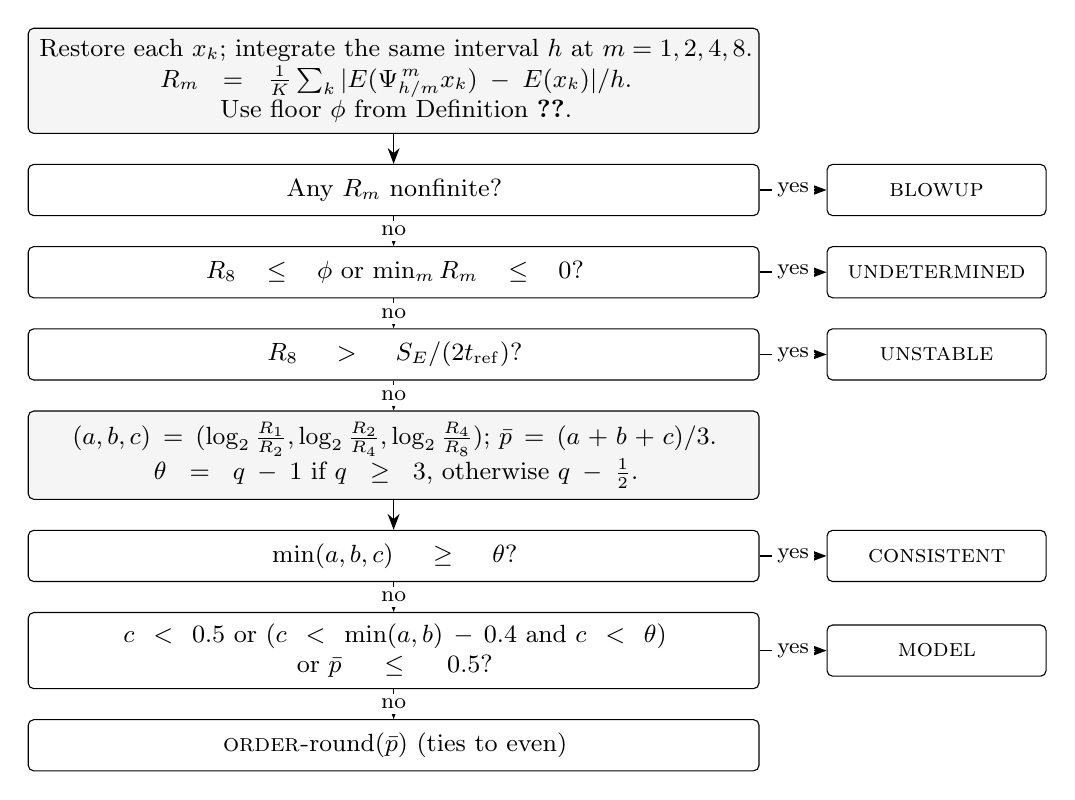
\begin{tikzpicture}[
  font=\small, >=Stealth,
  test/.style={draw,rounded corners=2pt,align=center,text width=9.0cm,
    minimum height=0.65cm,inner sep=4pt},
  exit/.style={draw,rounded corners=2pt,align=center,text width=2.5cm,
    minimum height=0.65cm,inner sep=4pt},
  flow/.style={->,semithick},
  lab/.style={font=\footnotesize,fill=white,inner sep=2pt}]
\node[test,fill=black!4] (sample) {Restore each $x_k$; integrate the same interval $h$ at $m=1,2,4,8$.\\
  $R_m=\frac1K\sum_k |E(\Psi_{h/m}^{\,m}x_k)-E(x_k)|/h$.\\Use floor $\phi$ from Definition~\ref{def:classifier}.};
\node[test,below=0.38cm of sample] (finite) {Any $R_m$ nonfinite?};
\node[exit,right=0.85cm of finite] (blowup) {\textsc{blowup}};
\node[test,below=0.38cm of finite] (floor) {$R_8\le\phi$ or $\min_m R_m\le0$?};
\node[exit,right=0.85cm of floor] (unresolved) {\textsc{undetermined}};
\node[test,below=0.38cm of floor] (large) {$R_8>S_E/(2t_{\mathrm{ref}})$?};
\node[exit,right=0.85cm of large] (unstable) {\textsc{unstable}};
\node[test,fill=black!4,below=0.38cm of large] (exponents) {
  $(a,b,c)=(\log_2\frac{R_1}{R_2},\log_2\frac{R_2}{R_4},\log_2\frac{R_4}{R_8})$; $\bar p=(a+b+c)/3$.\\
  $\theta=q-1$ if $q\ge3$, otherwise $q-\tfrac12$.};
\node[test,below=0.38cm of exponents] (consistent) {$\min(a,b,c)\ge\theta$?};
\node[exit,right=0.85cm of consistent] (pass) {\textsc{consistent}};
\node[test,below=0.38cm of consistent] (model) {$c<0.5$ or $(c<\min(a,b)-0.4\ \text{and}\ c<\theta)$\\
  or $\bar p\le0.5$?};
\node[exit,right=0.85cm of model] (fault) {\textsc{model}};
\node[test,below=0.38cm of model] (order) {\textsc{order-}$\operatorname{round}(\bar p)$ (ties to even)};
\draw[flow] (sample) -- (finite);
\draw[flow] (finite) -- node[lab]{no} (floor);
\draw[flow] (floor) -- node[lab]{no} (large);
\draw[flow] (large) -- node[lab]{no} (exponents);
\draw[flow] (exponents) -- (consistent);
\draw[flow] (consistent) -- node[lab]{no} (model);
\draw[flow] (model) -- node[lab]{no} (order);
\foreach \source/\target in {finite/blowup,floor/unresolved,large/unstable,consistent/pass,model/fault}
  \draw[flow] (\source) -- node[lab]{yes} (\target);
\end{tikzpicture}

\end{algorithm}

Matching exponents indicate conformance to the declared order; falling
exponents indicate a model fault; a lower plateau indicates an integrator
fault in the asymptotic regime. The fallback \emph{order-$k$} label
alone does not prove order reduction: its rounded mean can equal the
declared order even when one exponent fails the consistency threshold.
Ratios remove a common multiplicative defect scale across refinement levels.

\paragraph{Constants and provenance.}\label{sec:constants}
Refinement levels are fixed by design. Other constants were set during Acrobot
RK4 development; the archive lacks version history independently confirming
when they were fixed. Transfer and audits retain them unchanged.
Table~\ref{tab:sens} varies $\theta$, the finest-exponent threshold $0.5$,
the drop threshold $0.4$, and round-off factors $10,50,500$. Using
$\theta=q-0.5$ or $q-1$ for all $q$ also gives no healthy flags. MuJoCo
rigid bodies have small margins above the round-off floor. The noise factor
$5$ and large-defect threshold $S_E/(2t_{\mathrm{ref}})$ were not varied.

\subsubsection{From the theorem to the labels}\label{sec:bridge}

Theorem~\ref{thm:fp} is asymptotic in $h$ and requires $\beta_{q,q}\ne0$ for
the conserving-model order conclusion. At nonzero timestep sizes, guards and trajectory
averaging can suppress unresolved signals but give no error bound on the
label. Table~\ref{tab:failure} lists the failure modes and their experimental
evidence.

\begin{table}[htbp]
\centering\small
\begin{tabular}{>{\raggedright\arraybackslash}p{4.9cm}>{\raggedright\arraybackslash}p{4.2cm}>{\raggedright\arraybackslash}p{5.6cm}}
\toprule
Situation & Label returned & Evidence \\
\midrule
Asymptotic regime reached, finest residual above $\phi$ & informative (\emph{consistent}, \emph{model}, \emph{order-$k$}) & \S\ref{sec:exp:acrobot}--\ref{sec:exp:transfer} \\
Finest residual dominated by round-off or noise & \emph{undetermined} (never a fault) & no false alarm in any noise row (\S\ref{sec:exp:noise}); float32 readout abstains on every healthy run \\
Energy-preserving integrator & \emph{undetermined} & implicit midpoint, $40/40$ (\S\ref{sec:exp:transfer}) \\
Cancellation between finite-$h$ defect terms & spurious labels at one state; guarded trajectory scan abstains & sign change near $h\approx0.011$ (Appendix~\ref{app:cancellation}; \S\ref{sec:exp:finite}) \\
Model fault smaller than the truncation term (integrator error masks it) & \emph{order-$k$}, the dominant contribution & Euler $+1\%$ mass: order-1 $30/30$ (\S\ref{sec:exp:acrobot}) \\
Model fault that preserves $\Eref$ & undetected as model error; may pass or abstain & Proposition~\ref{prop:invariance} example \\
Declared order below / above the true order & \emph{consistent} / healthy runs flagged & RK4 declared $q=5$: $57/1000$ flagged; $q=6$: $1000/1000$ (\S\ref{sec:sens}) \\
Non-smooth step map (contacts, limits, state resets) & Lemma~\ref{lem:defect} does not apply; complete ungated test abstains in the contact study & Appendix~\ref{sec:audit:gate} \\
\bottomrule
\end{tabular}
\caption{Classifier failure modes, returned labels and experimental evidence.}
\label{tab:failure}
\end{table}

\paragraph{Deployment and follow-up.}\label{sec:deployment}
Freeze the invariant, parameters, energy units and offset. Restoring a state
must also restore time, caches, controller and random state. Use smooth passive
segments and archive the four residuals, exponents, floor, declared order and
software revision. For \emph{model}, check parameter caches and the invariant,
then repeat at smaller $h$ and additional starts. For \emph{order-$k$}, inspect
the integrator and state self-convergence. For \emph{undetermined}, check
precision, noise and exact energy preservation; enlarge $h$ only within a
credible smooth regime. For \emph{unstable}/\emph{blowup}, reduce $h$ and inspect
resets and constraints. Contacts require a separately justified regime gate.

When declared $q$ is unknown, report $(a,b,c)$ and their spread without a
\emph{consistent} label. A nonzero plateau suggests energy-defect order under
the theorem's visibility assumptions; noise can also give near-zero exponents.
No order-agnostic classifier is validated. Additional refinements can expose
curvature while approaching the noise floor; fitting a single power can
obscure $D+Tm^{-q}$, and alternative estimators remain untested. Changing
\texttt{frame\_skip} or thinning fixed-step logs changes the physical
interval, not integration resolution at fixed $h$, and cannot supply
Eq.~\eqref{eq:rm}. Since the residual is step-local, the trajectory horizon
changes the visited states rather than accumulating error (the horizon control
is in \S\ref{sec:exp:transfer}).

\section{Experimental setup}\label{sec:exp:setup}

The analytic Acrobot uses Gymnasium's \texttt{Acrobot-v1} parameters and
the energy function defined in Eq.~\eqref{eq:acrobot-energy}; the shipped-environment experiments use
\texttt{AcrobotEnv} and \texttt{CartPoleEnv} from Gymnasium 1.4.0
\citep{towers2024gymnasium} through \texttt{step} only, setting the step
attribute to $h/m$ and writing the float64 state. Unless stated, runs are
passive, noise-free float64, with the reference energy at nominal
parameters, and every experiment applies the float64 round-off guard
$\phi_{\mathrm{round}}$ of Definition~\ref{def:classifier} (only the
fixed-threshold baselines and the ``unguarded'' rows of the noise study in \S\ref{sec:exp:acrobot} run without it, by design).
Detection \emph{floors} are the smallest tested $\varepsilon$ from which all
larger tested values are detected. Within each fixed configuration, the
sampling unit is one random start state and intervals are $95\%$ Wilson
intervals. Starts are reused across step sizes, integrator orders and fault
levels in the finite-step and transfer studies. Pooled evaluation counts are
descriptive; they do not receive binomial intervals or rule-of-three bounds.
Table~\ref{tab:repeated} instead gives Wilson intervals for one binary outcome
per start, within each population, across its complete configuration grid.

\paragraph{Evaluation design and outcomes.}
Acrobot supplies development and shifted held-out starts; H\'enon--Heiles,
Kepler and the Euler top test transfer with unchanged constants. Unless stated,
faults perturb a physical parameter while energy retains its nominal value.
Sensitivity variants
and same-call self-convergence are post hoc.
An order-$k$ label with $k\ne q$ is an order-mismatch flag; order-$q$ is a
fallback label with no estimated order mismatch. A \emph{model} label on
conserving dynamics is a model-attribution error even if an integrator fault
is present. Coverage is the fraction receiving any non-abstaining label;
it is not classification accuracy.

\section{Results}\label{sec:results}

\subsection{Model error versus numerical error on Acrobot}\label{sec:validation}

\subsubsection{Reference-free classification on the shipped Acrobot}\label{sec:exp:acrobot}

We apply Definition~\ref{def:classifier} ($q=4$) to the shipped
\texttt{AcrobotEnv} at $\Delta t=0.2$, 10~s trajectories, start states
uniform on $[-1.5,1.5]^4$. The shipped step agrees with the analytic RK4
step to $2.8\times10^{-17}$ at the single state $(0.1,-0.2,0.3,-0.15)$.
For $1000$ uniform starts on $[-1.5,1.5]^4$ (seed 0), the maximum absolute
component difference per step has median $2.22\times10^{-16}$ and maximum
$8.88\times10^{-16}$ (\texttt{acrobot\_step\_agreement.csv}). Faults are injected into the real object: a
parameter attribute $\times(1+\varepsilon)$, a patched \texttt{rk4}
(Euler or midpoint), or \texttt{book\_or\_nips}$=$\texttt{"nips"} (the
variant that drops a Coriolis term). \texttt{LINK\_LENGTH\_2} is never read by
\texttt{AcrobotEnv} and is excluded as a null fault.

\paragraph{False alarms and exponents.} All $1000$ healthy runs are
classified \emph{consistent} (95\% upper bound on the false-alarm rate by the
rule of three: $0.3\%$). The round-off guard never binds here: on the
$150$ healthy runs of the fingerprint benchmark the finest residual exceeds $\phi_{\mathrm{round}}$ by a median factor of
$3.5\times10^{6}$ and by at least $1.5\times10^{4}$. The exponent distribution is shown in Figure~\ref{fig:fp2}.

\paragraph{Calibrated fixed-threshold detectors.}
Thresholds calibrated as the maximum over 100 healthy runs give held-out
false alarms of $0/100$ (energy drift), $4/100$ (raw $r$), $6/100$
(8 sub-steps) and $0/100$ ($R_2$). At $\varepsilon=10^{-4}$ on
\texttt{LINK\_MASS\_1}, calibrated $R_2$ detects $15/40$, against $40/40$
classified \emph{model} by the fingerprint.

\begin{table}[htbp]
\centering\small
\begin{tabular}{>{\raggedright\arraybackslash}p{5.4cm}>{\raggedright\arraybackslash}p{8.6cm}}
\toprule
Case (30 starts each) & Class assigned \\
\midrule
Healthy (1000) & consistent $1000$ \\
6 parameters, $\varepsilon\in\{10^{-4},10^{-3},10^{-2}\}$ & model $30/30$ in every cell \\
6 parameters, $\varepsilon=10^{-5}$ & model $30/30$ for \texttt{MASS\_2}, \texttt{LENGTH\_1}, \texttt{COM\_POS\_2}, \texttt{MOI}; $29/30$ \texttt{MASS\_1}; $26/30$ \texttt{COM\_POS\_1} \\
Catalogue: $m_2{=}1.3$, $l_1{=}1.2$, $l_{c2}{=}0.6$, $I{=}1.5$ (both links) & model $25,28,27,26$ of $30$; remaining $5,2,3,4$ unstable \\
Catalogue: \texttt{nips} (Coriolis dropped) & model $19/30$, unstable $11/30$ \\
Catalogue: Euler & order-1 $30/30$ \\
Midpoint RK2 & order-2 $20$, order-3 $8$, model $1$, consistent $1$ \\
Euler $+\,m_2{+}10^{-2}$ & order-1 $30/30$ (model fault masked) \\
Euler $+\,m_2{+}1$ & unstable $30/30$ (large-defect-rate abstention) \\
RK2 $+\,m_2{+}10^{-2}$ and $+10^{-1}$ & model $30/30$ each \\
\bottomrule
\end{tabular}
\caption{Fingerprint classes on the shipped Acrobot with both floors and the
large-defect-rate guard. Large catalogue faults can trigger abstention even
when their unguarded exponents indicate a model fault. In the Euler
$m_2{+}1$ case, $15/30$ starts encounter velocity clipping; that row includes
non-smooth transitions outside the refinement theorem's assumptions.}
\label{tab:I}
\end{table}

\begin{figure}[htbp]
\centering
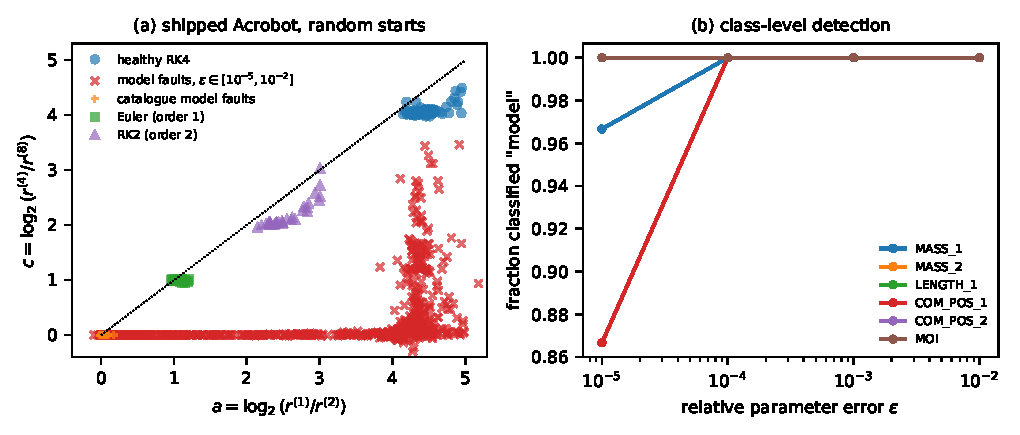
\includegraphics[width=0.98\linewidth]{fig/fig_fingerprint2.pdf}
\caption{(a) Exponents $a$ and $c$ per start state: healthy runs cluster near
$(4.4,4.0)$; model faults first lose the finest exponent $c$ (the vertical
column near $a\approx4.4$) and then $a$, ending near the origin. Points include candidates on which
the guard abstains; exponents alone do not determine the final label. Euler sits at
$(1,1)$ and RK2 near $2$. (b) Fraction classified model versus
$\varepsilon$.}
\label{fig:fp2}
\end{figure}

\paragraph{Class-level floor.} The fraction classified \emph{model} (30 starts)
at $\varepsilon=10^{-7},10^{-6},3\times10^{-6},10^{-5}$ is $1,14,26,30$ for
\texttt{MASS\_2} and \texttt{MOI}, $0,10,23,30$ for \texttt{LENGTH\_1}, and
$0,1,7,26$ for \texttt{COM\_POS\_1}, with no detections at $10^{-8}$ or below.
The class-level floor is therefore about $10^{-6}$--$10^{-5}$, with zero
false alarms.

\paragraph{Noise and the guard.} With independent noise on every energy
evaluation, healthy runs at $\sigma_E=10^{-6}$ are labelled \emph{model} for
$37/60$ starts without the guard, because the noise floor of the residual
mimics a nonvanishing defect; with the guard of
Definition~\ref{def:classifier} they become \emph{undetermined} ($59/60$) and
there are no false alarms. With the guard, a model fault at $m_2{+}10^{-4}$ is
still classified model at $\sigma_E=10^{-6}$ ($30/30$) and becomes
undetermined at $10^{-4}$; Euler is classified order-1 at every tested
noise level. Section~\ref{sec:exp:noise} separates noise sources and describes
how the guard's energy-error scale is obtained.

\paragraph{Masking.} An integrator error can hide a model error: Euler with
$m_2{+}10^{-2}$ is labelled order-1, since the Euler defect ($\approx0.3$) is
far above the model rate ($\approx0.2\varepsilon$), whereas an order-2
integrator does not mask a $1\%$ model fault. The class label reports the
\emph{dominant} contribution.

\subsubsection{Finite-step validation of the frozen classifier}\label{sec:exp:finite}

We test the classifier of Algorithm~\ref{alg:classifier} without retuning, using generic
Runge--Kutta integrators of order $q=1,2,3,4$, declared order equal to the true
order, on development starts (uniform on $[-1.5,1.5]^4$) and on \emph{held-out}
starts from a shifted distribution (angles uniform on $[-\pi,\pi]$, velocities on
$[-3,3]$), at $h=0.05,0.1,0.2$, with $\varepsilon\in\{0,10^{-4},\dots,10^{-1}\}$
added to the second-link mass (so $\varepsilon>0$ is a mixed model-plus-integrator
fault); $40$ starts per cell, $2$~s trajectories, with the float64 round-off floor
as the guard.

\begin{table}[htbp]
\centering\small
\fittable{\begin{tabular}{rrrrrrr}
\toprule
Order $q$ & $h$ & healthy flagged & model rate $\varepsilon{=}10^{-4}$ & $10^{-3}$ & $10^{-2}$ & $10^{-1}$ \\
\midrule
1 & 0.05 & 0/40 & 0.00 [0.00,0.09] & 0.00 [0.00,0.09] & 0.00 [0.00,0.09] & 0.93 [0.80,0.97] \\
1 & 0.1 & 0/40 & 0.00 [0.00,0.09] & 0.00 [0.00,0.09] & 0.00 [0.00,0.09] & 0.18 [0.09,0.32] \\
1 & 0.2 & 0/40 & 0.00 [0.00,0.09] & 0.00 [0.00,0.09] & 0.00 [0.00,0.09] & 0.03 [0.00,0.13] \\
2 & 0.05 & 0/40 & 0.48 [0.33,0.63] & 1.00 [0.91,1.00] & 1.00 [0.91,1.00] & 0.95 [0.83,0.99] \\
2 & 0.1 & 0/40 & 0.08 [0.03,0.20] & 0.95 [0.83,0.99] & 1.00 [0.91,1.00] & 0.95 [0.83,0.99] \\
2 & 0.2 & 0/40 & 0.00 [0.00,0.09] & 0.28 [0.16,0.43] & 1.00 [0.91,1.00] & 0.95 [0.83,0.99] \\
3 & 0.05 & 0/40 & 1.00 [0.91,1.00] & 1.00 [0.91,1.00] & 1.00 [0.91,1.00] & 0.95 [0.83,0.99] \\
3 & 0.1 & 0/40 & 1.00 [0.91,1.00] & 1.00 [0.91,1.00] & 1.00 [0.91,1.00] & 0.95 [0.83,0.99] \\
3 & 0.2 & 0/40 & 0.18 [0.09,0.32] & 1.00 [0.91,1.00] & 1.00 [0.91,1.00] & 0.98 [0.87,1.00] \\
4 & 0.05 & 0/40 & 1.00 [0.91,1.00] & 1.00 [0.91,1.00] & 1.00 [0.91,1.00] & 0.95 [0.83,0.99] \\
4 & 0.1 & 0/40 & 1.00 [0.91,1.00] & 1.00 [0.91,1.00] & 1.00 [0.91,1.00] & 0.95 [0.83,0.99] \\
4 & 0.2 & 2/40 & 1.00 [0.91,1.00] & 1.00 [0.91,1.00] & 1.00 [0.91,1.00] & 0.98 [0.87,1.00] \\
\bottomrule
\end{tabular}
}
\caption{Held-out starts: healthy runs flagged, and the model rate with its
$95\%$ Wilson interval, for an integrator of true order $q$.}
\label{tab:finitestep}
\end{table}

No healthy evaluation was labelled model in either set ($0/480$ development, $0/480$ held-out; $40$ starts reused across $12$ configurations per set); $2/480$
held-out evaluations were RK4 runs at $h=0.2$ labelled \emph{order-4}, near the
\emph{consistent} boundary ($2/40$ starts in that configuration). This fallback
label rounds the mean exponent to $4$, but at least one exponent fails the
\emph{consistent} threshold; it does not establish order reduction.
The masking boundary moves with order and step size
(Table~\ref{tab:finitestep}): Euler often masks even a $10\%$ mass error,
whereas RK4 detects every tested error from $10^{-4}$ through $10^{-2}$.
Some $10\%$ faults instead trigger the
large-defect-rate guard, reducing detection to $38$--$39$ of $40$ held-out
RK4 starts ($0.950$--$0.975$). \emph{Degenerate states.} Starting within $10^{-3}$ of
equilibrium the RK4 defect is below the float64 floor and the classifier returns \emph{undetermined} for $40/40$ starts at every $h$; for $q=2,3$ the healthy runs abstain only partly ($14/40$ and $31/40$ at $h=0.05$, none at $h=0.2$).
A model error of $10^{-2}$ is detected in $40/40$ runs for every $q\ge2$ and every $h$, including the RK4 runs whose healthy
counterpart abstains, and is masked for $q=1$.
\emph{Sign change.} On one start state and one step, healthy RK4 swept over $h$ shows the failure mode of the
asymptotic argument (Figure~\ref{fig:sign}): without a floor the labels become model at $h\approx0.043,0.033$ and then scatter between
order-4, 3, 2 and undetermined at $h\le0.026$; with the float64 floor every $h\le0.043$ is undetermined. The experimental protocol therefore withholds labels below the floor and
uses trajectory means evaluated over multiple starts, subject to the
finite-step limits in \S\ref{sec:bridge}.

\subsection{Comparison with alternative diagnostics}\label{sec:position}

\subsubsection{Invariant-defect extrapolation and raw drift}\label{sec:extrap-main}

Invariant-defect extrapolation is a direct alternative using the same
invariant and refined step map. The established Richardson construction
\citep{richardson1927} cancels leading truncation terms; Appendix~\ref{app:extrap}
derives the order-adapted weights. We compare the trajectory mean of
$|R_2|$ with raw residuals, eight-sub-step residuals, energy standard
deviation and the fingerprint on shipped passive Acrobot. Each scalar
threshold is the maximum of $100$ healthy calibration starts. All methods
use the same $100$ held-out healthy starts and the same $40$ candidate
starts within each fault configuration. The fingerprint uses its existing
constants and no healthy-run threshold. The fault seed changes between
configurations; counts are paired within each row, not across rows.

\begin{table}[htbp]
\centering\small
\fittable{\begin{tabular}{lrrrrrr}
\toprule
Candidate & $n$ & drift flag & raw flag & sub8 flag & $R_2$ flag & fingerprint model \\
\midrule
healthy (held-out) & 100 & 0 & 4 & 6 & 0 & 0 \\
mass 1 $+10^{-6}$ & 40 & 0 & 0 & 2 & 0 & 0 \\
mass 1 $+10^{-5}$ & 40 & 0 & 0 & 20 & 0 & 38 \\
mass 1 $+10^{-4}$ & 40 & 1 & 2 & 39 & 15 & 40 \\
Euler & 40 & 40 & 40 & 40 & 40 & 0 \\
midpoint RK2 & 40 & 37 & 37 & 40 & 40 & 0 \\
Euler + mass 2 $+1\%$ & 40 & 40 & 40 & 40 & 40 & 0 \\
\bottomrule
\end{tabular}
}
\caption{Existing calibrated-detector experiment at $h=0.2$, $10$~s,
with matched evaluation starts. Entries are counts. Scalar columns flag a
threshold exceedance; the final column counts \emph{model} labels, not all
fault flags. Thus zero in the final column for Euler or midpoint is not a
missed integrator fault: their full labels are order-1 and order-2/order-3.
The diagnostics require respectively $1$, $1$, $8$, $7$ and $15$ simulator
steps per sampled state, counting shared branches once; the trajectory
itself is shared. The $100$ calibration runs are additional baseline cost.}
\label{tab:extrap-main}
\end{table}

The extrapolated statistic reduces healthy truncation error, but still needs
a decision rule for its finite-step remainder. A threshold exceedance alone
does not distinguish changed dynamics from changed numerical order. The
fingerprint supplies a heuristic interpretation of the refinement pattern;
it does not introduce a new refinement or extrapolation principle. The
matched-compute studies in Appendix~\ref{app:extrap} also show that $R_2$
and plain sub-stepping have similar RK4 detection floors, while extrapolation
helps on the tested first-order CartPole integrator. Neither diagnostic is
uniformly more sensitive across these protocols.

\subsubsection{Reference-free state self-convergence at matched calls}\label{sec:selfconv}

To isolate what an invariant adds to state self-convergence
\citep{roache1998,nparcconvergence}, we compare both using the same endpoints
$X_m=\Psi_{h/m}^{\,m}(x)$, $m=1,2,4,8$. Define \[
d_m=\operatorname{mean}_k\|X_m(x_k)-X_{2m}(x_k)\|_2,\quad
p_{12}=\log_2(d_1/d_2),\qquad p_{24}=\log_2(d_2/d_4). \] Angular differences
are wrapped to $[-\pi,\pi]$, and the norm uses unit numerical weights for
angles in radians and velocities in radians per second. If
$X_m=\varphi_h^{f_c}(x)+C(h,x)m^{-q}+\cdots$ with a nonzero leading state
error, the common limiting flow cancels in the differences, yielding
$p_{12},p_{24}\to q$ in the asymptotic regime whether or not $f_c$ preserves
$E$. By contrast, the energy residual retains
$[E(\varphi_h^{f_c}(x))-E(x)]/h$, preserving the invariant-breaking signal
that state differences cancel.

This post-hoc control uses $40$ newly sampled starts (seed $20261104$), reused
across six Acrobot cases, two steps and $20$ macro-steps per start ($4$ s at $h=0.2$, $1$ s at
$h=0.05$). Both
measurements reuse the same $15$ simulator calls per macro-step; neither uses
a healthy trajectory or a finer reference solution. We freeze the existing
classifier and report self-convergence exponents without fitting a classifier
to them. We exclude clipped or nonfinite paths from both smooth diagnostics
and retain their counts; none occurs in these $480$ evaluations. A
$50\varepsilon_{\rm mach}(1+\max_m\|X_m\|)$ state-difference floor resolves
all starts. The protocol was fixed before running this post-hoc comparison.

\begin{table}[htbp]
\centering\small
\fittable{\begin{tabular}{lrcll}
\toprule
Candidate (declared $q=4$) & $h$ & Smooth / starts & State $p_{24}$ [10th, 90th] & Energy labels \\
\midrule
healthy RK4 & 0.2 & 40/40 & 4.02 [3.99, 4.06] & consistent 40 \\
healthy RK4 & 0.05 & 40/40 & 4.00 [3.97, 4.01] & consistent 40 \\
RK4 mass +0.1\% & 0.2 & 40/40 & 4.02 [3.99, 4.06] & model 40 \\
RK4 mass +0.1\% & 0.05 & 40/40 & 4.00 [3.97, 4.01] & model 40 \\
RK4 Coriolis omission & 0.2 & 40/40 & 4.04 [3.99, 4.08] & model 27, unstable 13 \\
RK4 Coriolis omission & 0.05 & 40/40 & 4.01 [4.00, 4.03] & model 36, unstable 4 \\
midpoint RK2 & 0.2 & 40/40 & 2.01 [1.98, 2.06] & order-2 35, order-3 4, model 1 \\
midpoint RK2 & 0.05 & 40/40 & 2.00 [1.99, 2.01] & order-2 37, model 2, order-3 1 \\
Euler & 0.2 & 40/40 & 1.02 [0.99, 1.06] & order-1 40 \\
Euler & 0.05 & 40/40 & 1.00 [0.99, 1.01] & order-1 40 \\
Euler mass +1\% & 0.2 & 40/40 & 1.02 [0.98, 1.08] & order-1 40 \\
Euler mass +1\% & 0.05 & 40/40 & 1.00 [0.99, 1.01] & order-1 40 \\
\bottomrule
\end{tabular}
}
\caption{Identical-call reference-free measurements on Acrobot. State entries
are median finest self-convergence exponents and between-start percentiles,
not confidence intervals. Energy entries use the frozen guarded classifier.
The $40$ starts are reused across rows.}
\label{tab:selfconv}
\end{table}

Table~\ref{tab:selfconv} shows state self-convergence close to order $4$ for
both healthy RK4 and RK4 with a $0.1\%$ mass error. The fingerprint labels
all $40$ mass-fault starts \emph{model} at each step size. With the Coriolis
omission, self-convergence still approaches $4$, while the energy rule labels
$27/40$ and $36/40$ starts \emph{model} at $h=0.2$ and $0.05$; the remaining
$13$ and $4$ receive the large-defect-rate abstention label. State
self-convergence correctly exposes midpoint and Euler order reduction. It is
also more precise here than the energy-based order label: midpoint with conserving dynamics
receives $1/40$ and $2/40$ spurious \emph{model} labels at the two steps, as
well as some order-3 labels.
For Euler plus a $1\%$ mass error, every energy label is order-1 at both
steps: the numerical error masks the model fault.

\begin{table}[htbp]
\centering\small
\fittable{\begin{tabular}{lrrrrrr}
\toprule
Candidate & consistent & model & order mismatch & order-$q$ & abstained & coverage \\
\midrule
healthy RK4, held-out ($h=0.2$) & 38/40 & 0/40 & 0/40 & 2/40 & 0/40 & 100.0\% \\
midpoint RK2 ($h=0.2$) & 0/40 & 1/40 & 39/40 & 0/40 & 0/40 & 100.0\% \\
midpoint RK2 ($h=0.05$) & 0/40 & 2/40 & 38/40 & 0/40 & 0/40 & 100.0\% \\
Euler mass +1\% ($h=0.2$) & 0/40 & 0/40 & 40/40 & 0/40 & 0/40 & 100.0\% \\
Euler mass +1\% ($h=0.05$) & 0/40 & 0/40 & 40/40 & 0/40 & 0/40 & 100.0\% \\
three transfer systems (pooled) & 1301/1440 & 0/1440 & 0/1440 & 0/1440 & 139/1440 & 90.3\% \\
\bottomrule
\end{tabular}
}
\caption{Distinct classifier outcomes in selected existing experiments.
Order mismatch counts order-$k$ with $k\ne q$; order-$q$ is the fallback
without estimated mismatch. The dynamics integrated by midpoint conserve
the specified energy, so its model labels are erroneous attributions.
Euler plus a mass fault illustrates masking: an order flag
does not imply correct model-fault attribution. Coverage includes erroneous
labels. Each Acrobot row uses $40$ starts, reused across timesteps within
its experiment; transfer counts are $1440$ evaluations of $120$ starts.}
\label{tab:diagnostic-outcomes}
\end{table}

\subsubsection{Matched-step and direct-reference controls}\label{sec:exp:K}

We apply the exact permutation test of \citet{gebrekidan2026diagnosing} to the refinement statistics, on its
analytic Acrobot, its eight paired initial conditions (seed $0$), $\alpha=0.01$, fault $m_2\to m_2(1+\varepsilon)$, noise-free. The permutation test is an \emph{unpaired two-sample} test with
$n=8$ per arm and minimum achievable $p\approx7.8\times10^{-5}$. The
detection floor depends on effect size, between-start variation and the
numerical threshold.
Table~\ref{tab:K} compares detection floors at the same macro-step and at
matched simulator step sizes, with a direct reference-step baseline.

\begin{table}[htbp]
\centering\small
\fittable{\begin{tabular}{rcccccccc}
\toprule
 & \multicolumn{4}{c}{reference-based screen, simulator step} & \multicolumn{2}{c}{refinement at $\Delta t$} & & \\
\cmidrule(lr){2-5}\cmidrule(lr){6-7}
$\Delta t$ & $\Delta t$ & $\Delta t/2$ & $\Delta t/4$ & $\Delta t/8$ & 8 sub-steps & $R_2$ & raw $r^{(1)}$ & \shortstack{direct reference\\step comparison} \\
\midrule
0.2 & $10^{-1}$ & $10^{-2}$ & $10^{-4}$ & $10^{-5}$ & $10^{-5}$ & $10^{-5}$ & $10^{-2}$ & $10^{-13}$ \\
0.1 & $10^{-2}$ & $10^{-4}$ & $10^{-5}$ & $10^{-7}$ & $10^{-7}$ & $10^{-7}$ & $10^{-3}$ & $10^{-13}$ \\
0.05 & $10^{-4}$ & $10^{-5}$ & $10^{-7}$ & $10^{-8}$ & $10^{-8}$ & $10^{-9}$ & $10^{-4}$ & $10^{-13}$ \\
0.01 & $10^{-7}$ & -- & -- & -- & $10^{-10}$ & $10^{-12}$ & $10^{-7}$ & -- \\
0.005 & $10^{-8}$ & -- & -- & -- & $10^{-11}$ & $10^{-12}$ & $10^{-8}$ & -- \\
\bottomrule
\end{tabular}
}
\caption{Detection floors (relative $m_2$ error), same permutation test and initial conditions. The screen's absolute
floor $10^{-8}$ is shown (a float64-level floor $10^{-14}$ changes only the $\Delta t=0.005$ entry, $10^{-9}$). Horizons are
$10$~s for $\Delta t\ge0.05$, $4$~s at $0.01$ and $2$~s at $0.005$. Floors at $\Delta t=0.01,0.005$ are censored at the grid
minimum $10^{-12}$. ``Direct step compare'': largest state difference between the faulty and nominal simulator after one step
exceeds $10^{-14}$.}
\label{tab:K}
\end{table}

At the same macro-step, the refinement statistics detect faults $3$ to $5$
decades below the screen. They use calls at $\Delta t/8$; running the screen
at that finer step reaches the same floors ($10^{-5}$ at $\Delta t=0.2$,
$10^{-7}$ at $0.1$, within one decade at $0.05$). Direct comparison of a
faulty and nominal step reaches $10^{-13}$ at every tested $\Delta t$
($0.2$, $0.1$, $0.05$), four to eight decades below the refinement statistics.
In this comparison, reference-based methods provide equal or greater
sensitivity when nominal dynamics are available. The fingerprint supplies fault-class
information using an invariant and the candidate step map. The same access
also permits the parameter fit in Appendix~\ref{app:ident}.

The screen uses logged observations and tolerates float32; the fingerprint
requires the access in \S\ref{sec:setting}. This comparison covers one mass
fault without noise and excludes the screen's localisation and attribution
stages. Its published $m_2$ floor at observation noise $10^{-3}$ is $10^{-1}$;
a comparison in those noise units was not run.

\subsection{Transfer and robustness}\label{sec:robustness}

\subsubsection{Transfer to systems not used in development}\label{sec:exp:transfer}

We apply the same constants, threshold rule and round-off factor to
Runge--Kutta integrators of order $q=1,\dots,4$
on three further systems with a coupling, gravitational-parameter or inertia
fault of relative size $\varepsilon$ ($\Eref$ at the nominal value), $40$ starts
per cell and three step sizes each:
H\'enon--Heiles; planar Kepler orbits; and a free rigid body (Euler top, a
Lie--Poisson system with $I=(1,2,3)$ and fault $I_3\to3(1+\varepsilon)$). The
third system was added after the first two and its protocol (starts, steps,
horizon, orders) was fixed in the benchmark's docstring before it was run.

\begin{table}[htbp]
\centering\small
\fittable{\begin{tabular}{llrrrrr}
\toprule
System & $q$ & healthy flagged & healthy abstained & model $\varepsilon{=}10^{-4}$ & $10^{-3}$ & $10^{-2}$ \\
\midrule
H\'enon--Heiles & 1 & 0/120 & 108/120 & 0.00 & 0.00 & 0.01 \\
 & 2 & 0/120 & 0/120 & 0.44 & 0.99 & 1.00 \\
 & 3 & 0/120 & 0/120 & 0.68 & 1.00 & 1.00 \\
 & 4 & 0/120 & 0/120 & 1.00 & 1.00 & 1.00 \\
\addlinespace
Kepler & 1 & 0/120 & 0/120 & 0.00 & 0.00 & 0.00 \\
 & 2 & 0/120 & 0/120 & 0.61 & 1.00 & 1.00 \\
 & 3 & 0/120 & 0/120 & 0.94 & 1.00 & 1.00 \\
 & 4 & 0/120 & 2/120 & 1.00 & 1.00 & 1.00 \\
\addlinespace
Euler top & 1 & 0/120 & 0/120 & 0.00 & 0.00 & 0.11 \\
 & 2 & 0/120 & 0/120 & 0.79 & 1.00 & 1.00 \\
 & 3 & 0/120 & 0/120 & 1.00 & 1.00 & 1.00 \\
 & 4 & 0/120 & 29/120 & 1.00 & 1.00 & 1.00 \\
\bottomrule
\end{tabular}
}
\caption{Same classifier constants on three further systems. Each row pools
$120$ evaluations of $40$ starts at three step sizes. Healthy flagged means
any non-consistent, non-abstaining label. Model rates are descriptive pooled
rates without pooled confidence intervals. The accompanying result files
provide separate per-step rates and $95\%$ Wilson intervals.}
\label{tab:transfer}
\end{table}

No healthy run in any of the $36$ (system, order, step) cells was labelled model or order-$k$:
$0/1440$ evaluations of $120$ system-specific starts. There are $1301$
consistent labels and $139$ abstentions (coverage $90.3\%$). For each system,
$0/40$ starts receive any fault flag across the $12$ configurations; the
start-level $95\%$ Wilson upper bound is $8.8\%$ (Table~\ref{tab:repeated}).
For every order $q\ge2$ an error of $10^{-2}$ is labelled
\emph{model} in all $1080/1080$ runs, and for RK4 an error of $10^{-4}$ in $360/360$. At $q=2$, H\'enon--Heiles has the lowest pooled model rate at a $10^{-4}$
error ($0.44$). At $10^{-3}$, all pooled system/order rates for $q\ge2$
are at least $0.99$; the minimum individual step-specific rate is
$39/40$ ($0.975$). For Euler ($q=1$) the
truncation term masks the model fault, as in \S\ref{sec:exp:acrobot}, except that the Euler top with a $10^{-2}$ error is labelled
model in $11\%$ of runs. Abstentions are confined to three places: H\'enon--Heiles with Euler ($108/120$ healthy runs are
\emph{unstable} or blow up at the larger steps), the RK4 Euler top ($29/120$, finest residual at the round-off floor), and Kepler
with RK4 ($2/120$). \emph{Horizon.} H\'enon--Heiles at $h=0.1$ gives identical labels at $T=20$ and $T=200$ (healthy
\emph{consistent} in $20/20$ and a $10^{-3}$ error labelled \emph{model} in $20/20$, for $q=2$ and $q=4$), consistent with the
step-local nature of the residual.

\emph{Energy-preserving integrators.} For the implicit midpoint rule on a
harmonic oscillator, which conserves the quadratic energy exactly, the finest
residual is round-off and the classifier returns \emph{undetermined} in $40/40$
runs at $h=0.1,0.4,1.0$, as predicted by Remark~\ref{rem:conserving}.

\subsubsection{Noise sources and the operating envelope}\label{sec:exp:noise}

We separate four noise sources on
the analytic Acrobot at $h=0.2$ ($40$ random starts, $10$~s, the frozen
classifier). \emph{Start-state noise}: the diagnostic start is a noisy logged
observation, but the simulator is re-stepped from it and energies are exact.
\emph{Readout noise}: every state read back for an energy evaluation (the start
and each refined end state) carries independent noise, as for a noisy observation
channel on the simulator's output. \emph{Energy-evaluation noise}: independent
noise on each energy value. \emph{float32 readout}: the four internal state
coordinates are rounded to float32. This tests internal-state quantisation;
Gymnasium's six-component trigonometric observation map is not used.
Integration and round-off error of the step map
itself is the noise-free float64 row. The guard's energy-error scale is
estimated from repeated independent readouts of fixed states. For the
deterministic float32 quantiser we instead use the declared precision with
$\pm\tfrac12$ ulp dithering as a sensitivity model. Repeated identical
quantised reads give no estimate of rounding error. A conservative alternative
uses rounding cells to bound the endpoint energy errors by $B_0,B_1$, giving
residual uncertainty at most $(B_0+B_1)/h$ and requiring abstention when the
exponents are unresolved. These bounds were not tested as an additional noise
experiment. A fault is detected if labelled model.

\begin{table}[htbp]
\centering\small
\fittable{\begin{tabular}{llrrrr}
\toprule
Source & $\sigma$ & healthy flagged / undet. & model $\varepsilon{=}10^{-4}$ & $10^{-3}$ & $10^{-2}$ \\
\midrule
float64 (no added noise) & -- & 0.00 / 0.00 & 1.00 (0.00) & 1.00 (0.00) & 1.00 (0.00) \\
start-state noise & $10^{-8}$ & 0.00 / 0.00 & 1.00 (0.00) & 1.00 (0.00) & 1.00 (0.00) \\
start-state noise & $10^{-6}$ & 0.00 / 0.00 & 1.00 (0.00) & 1.00 (0.00) & 1.00 (0.00) \\
start-state noise & $10^{-5}$ & 0.00 / 0.00 & 1.00 (0.00) & 1.00 (0.00) & 1.00 (0.00) \\
start-state noise & $10^{-4}$ & 0.00 / 0.00 & 1.00 (0.00) & 1.00 (0.00) & 1.00 (0.00) \\
start-state noise & $10^{-3}$ & 0.00 / 0.00 & 1.00 (0.00) & 1.00 (0.00) & 1.00 (0.00) \\
readout state noise & $10^{-8}$ & 0.00 / 0.68 & 1.00 (0.00) & 1.00 (0.00) & 1.00 (0.00) \\
readout state noise & $10^{-6}$ & 0.00 / 1.00 & 0.82 (0.17) & 1.00 (0.00) & 1.00 (0.00) \\
readout state noise & $10^{-5}$ & 0.00 / 1.00 & 0.00 (1.00) & 0.80 (0.20) & 1.00 (0.00) \\
readout state noise & $10^{-4}$ & 0.00 / 1.00 & 0.00 (1.00) & 0.00 (1.00) & 0.82 (0.17) \\
readout state noise & $10^{-3}$ & 0.00 / 1.00 & 0.00 (1.00) & 0.00 (1.00) & 0.00 (1.00) \\
energy-evaluation noise & $10^{-8}$ & 0.00 / 0.15 & 1.00 (0.00) & 1.00 (0.00) & 1.00 (0.00) \\
energy-evaluation noise & $10^{-6}$ & 0.00 / 1.00 & 1.00 (0.00) & 1.00 (0.00) & 1.00 (0.00) \\
energy-evaluation noise & $10^{-5}$ & 0.00 / 1.00 & 0.68 (0.33) & 1.00 (0.00) & 1.00 (0.00) \\
energy-evaluation noise & $10^{-4}$ & 0.00 / 1.00 & 0.00 (1.00) & 0.68 (0.33) & 1.00 (0.00) \\
energy-evaluation noise & $10^{-3}$ & 0.00 / 1.00 & 0.00 (1.00) & 0.00 (1.00) & 0.65 (0.35) \\
float32 readout & -- & 0.00 / 1.00 & 1.00 (0.00) & 1.00 (0.00) & 1.00 (0.00) \\
\bottomrule
\end{tabular}
}
\caption{Operating envelope. Entries are the fraction of $40$ starts labelled
model, with the fraction labelled undetermined in parentheses; the healthy
column is the fraction flagged as non-consistent and the fraction
undetermined. A rate of $0.80$--$0.82$ has a $95\%$ Wilson interval of about
$[0.66,0.91]$.}
\label{tab:noisesrc}
\end{table}

(i) Start-state noise has no effect up to $\sigma=10^{-3}$: noise only moves the evaluation point of a
smooth function. (ii) Readout noise is the harmful channel and is roughly an order of magnitude worse than
energy-evaluation noise at the same $\sigma$ (for $\sigma=10^{-5}$ the model rate at $\varepsilon=10^{-3}$ is $0.80$ for
readout noise and $1.00$ for energy noise; at $\varepsilon=10^{-4}$ it is $0.00$ against $0.68$), as expected if readout
noise is amplified by the energy's gradient, which is of order $10$ here. (iii) The guard produced no healthy false alarm
in any condition ($0/40$ flagged in all $17$ rows); beyond the envelope the method abstains, and float32 readout abstains
on every healthy run while still flagging faults of $10^{-4}$ and above. The smallest tested $\varepsilon$ with model rate
$\ge0.8$ rises from $\le10^{-4}$ in float64 to $10^{-4}$, $10^{-3}$, $10^{-2}$ and above $10^{-2}$ for readout noise
$10^{-6},10^{-5},10^{-4},10^{-3}$, on a grid of three values. (iv) The fixed-gate paired baselines (raw, 8 sub-steps,
$R_2$; flagged above ten times a paired healthy run under independent noise) lose detection of $\varepsilon=10^{-3}$ at
$\sigma=10^{-5}$ readout noise ($0.15$--$0.20$ against $0.80$ for the classifier); their gate was not tuned, so this is a
comparison of procedures, not of the best possible thresholds. The abstention is one-sided: at the tested readout-noise levels
$\sigma\ge10^{-6}$ (standard deviation per state component, in radians for angles
and radians per second for angular velocities), and in the float32 internal-state
readout test, the healthy column is entirely \emph{undetermined}, so the method can
flag faults in that regime but cannot certify health. These tests cover
independent Gaussian noise and deterministic float32 quantisation on Acrobot.

\subsubsection{Sensitivity to the constants and to a misdeclared order}\label{sec:sens}

Table~\ref{tab:sens} re-scores stored residuals under variants of the
classifier constants on Acrobot and the three transfer systems, including the
round-off factor. The default rule is retained.

\begin{table}[htbp]
\centering\small
\fittable{\begin{tabular}{lrrrrrrr}
\toprule
 & \multicolumn{2}{c}{Acrobot RK4 (development)} & \multicolumn{5}{c}{Three transfer systems} \\
\cmidrule(lr){2-3}\cmidrule(lr){4-8}
Variant & healthy model & faults $10^{-5}$ & healthy model & healthy other flag & healthy abstain & faults $10^{-2}$ & HH faults $10^{-4}$ \\
\midrule
default (as in the paper) & 0/1000 & 175/180 & 0/1440 & 0 & 139 & 1080/1080 & 254/360 \\
$c_{\mathrm{thr}}=0.25$ & 0/1000 & 175/180 & 0/1440 & 0 & 139 & 1080/1080 & 254/360 \\
$c_{\mathrm{thr}}=1.0$ & 0/1000 & 175/180 & 0/1440 & 0 & 139 & 1080/1080 & 254/360 \\
$\delta=0.1$ & 0/1000 & 175/180 & 0/1440 & 0 & 139 & 1080/1080 & 254/360 \\
$\delta=0.8$ & 0/1000 & 175/180 & 0/1440 & 0 & 139 & 1080/1080 & 254/360 \\
$\theta=q-0.5$ (all $q$) & 0/1000 & 180/180 & 0/1440 & 0 & 139 & 1080/1080 & 270/360 \\
$\theta=q-1$ (all $q$) & 0/1000 & 175/180 & 0/1440 & 0 & 139 & 1080/1080 & 241/360 \\
$\theta=q-1.5$ (all $q$) & 0/1000 & 166/180 & 0/1440 & 0 & 139 & 1080/1080 & 239/360 \\
round-off factor 10 & 0/1000 & 175/180 & 0/1440 & 0 & 127 & 1080/1080 & 254/360 \\
round-off factor 500 & 0/1000 & 175/180 & 0/1440 & 0 & 175 & 1080/1080 & 254/360 \\
\bottomrule
\end{tabular}
}
\caption{Variants of the decision rule. Healthy model: healthy runs labelled
\emph{model}; healthy other flag: labelled \emph{order-$k$}; healthy abstain:
\emph{undetermined}, \emph{unstable} or \emph{blowup}. Faults on the transfer
systems are $\varepsilon=10^{-2}$ for $q=2,3,4$; HH adds weak
H\'enon--Heiles faults at $10^{-4}$ for the same orders.}
\label{tab:sens}
\end{table}

None of the ten settings flags a healthy Acrobot or
transfer evaluation (Table~\ref{tab:sens}). For weak H\'enon--Heiles faults at $10^{-4}$ (orders 2--4, $360$
reused-start evaluations), the default detects $254/360$; the $\theta$
variants detect $239$--$270/360$, and the other variants retain $254/360$.
Threshold changes affect the weakest
Acrobot faults; round-off factors $10$, $50$ and $500$ change healthy transfer
abstentions to $127$, $139$ and $175$ of $1440$, while retaining all tested
$1\%$ faults at orders $2$--$4$. The Euler label is sensitive to
$c_{\mathrm{thr}}$: only $7/30$ runs remain order-1 at $1.0$, and none at
$1.5$. RK2's order label also depends on $\delta$. The noise factor $5$ and
the large-defect-rate threshold were not varied.

\emph{Misdeclaring the order.} A consistent label means that the measured
energy-defect exponents clear the declared-order threshold; it does not
certify trajectory order.
Declaring a lower order than the true one passes (RK4 declared as $q=2$ or $3$ is
\emph{consistent}); declaring a higher one flags healthy runs ($q=5$: $57/1000$;
$q=6$: $1000/1000$). The order-$k$ label is accurate to about one order (RK2 is
labelled order-2 in $20/30$ runs, order-3 in $8/30$, and once each \emph{model} and
\emph{consistent}); using the finest exponent $c$ alone instead of the mean of
$(a,b,c)$ changes the RK2 order-2 count from $20/30$ to $25/30$.
For healthy RK4, the fraction whose rounded exponent estimate equals 4 changes
from $955/1000$ to $986/1000$; these are auxiliary order estimates, while
the classifier labels all $1000$ runs \emph{consistent}. Equal-order integrators are indistinguishable.

\subsubsection{Repeated-start uncertainty}\label{sec:exp:summary}

The evaluation counts above reuse starts across configurations. Table~\ref{tab:repeated}
reports one outcome per start, with within-population Wilson intervals,
rather than treating the pooled evaluations as independent samples.

\begin{table}[htbp]
\centering\small
\fittable{\begin{tabular}{llrrr}
\toprule
Population & Start-level endpoint & $k/n$ starts & configurations & 95\% Wilson \\
\midrule
Euler top & any healthy fault flag & 0/40 & 12 & [0.000,0.088] \\
Euler top & $1\%$ fault: all model & 40/40 & 9 & [0.912,1.000] \\
H\'enon--Heiles & any healthy fault flag & 0/40 & 12 & [0.000,0.088] \\
H\'enon--Heiles & $1\%$ fault: all model & 40/40 & 9 & [0.912,1.000] \\
Kepler & any healthy fault flag & 0/40 & 12 & [0.000,0.088] \\
Kepler & $1\%$ fault: all model & 40/40 & 9 & [0.912,1.000] \\
Acrobot development & any healthy fault flag & 0/40 & 12 & [0.000,0.088] \\
Acrobot development & $1\%$ fault: all model & 40/40 & 9 & [0.912,1.000] \\
Acrobot held-out & any healthy fault flag & 2/40 & 12 & [0.014,0.165] \\
Acrobot held-out & $1\%$ fault: all model & 40/40 & 9 & [0.912,1.000] \\
\bottomrule
\end{tabular}
}
\caption{One binary endpoint per start across its configuration grid.
``Any healthy fault flag'' includes model and order-$k$ labels but excludes
abstentions. ``All model'' requires the $1\%$ fault to be labelled model in
every order-$2$--$4$, step-size configuration. Each population has $40$
independently sampled starts; intervals concern new starts in that population,
not new systems.}
\label{tab:repeated}
\end{table}

\subsection{Simulator audits}\label{sec:audits}

\subsubsection{Domain-randomisation consistency}\label{sec:audit:dr}

Domain randomisation sets attributes by assignment
(\texttt{env.unwrapped.attr = value}) every episode. For each attribute of
Gymnasium's Acrobot, CartPole and Pendulum, at factors $0.5,1.0,1.5,2.0$, we
set it that way and test whether the simulator still conserves the energy
built from its \emph{own} declared attribute values (24--40 random starts per
cell; passive; declared $q=4,1,1$). Where an environment caches derived
constants (CartPole's \texttt{total\_mass}, \texttt{polemass\_length}) we also
test the fully updated variant (Table~\ref{tab:dr}).

\begin{table}[htbp]
\centering\small
\fittable{\begin{tabular}{llll}
\toprule
Environment & Attribute & Assigned directly & Cached constants updated \\
\midrule
CartPole & \texttt{masscart} & model $40/40$ at $\times0.5,1.5,2$; \emph{no-op} & consistent $40/40$ \\
CartPole & \texttt{masspole} & model $40/40$ at $\times0.5,1.5,2$ & consistent $40/40$ \\
CartPole & \texttt{length} & model $40/40$ at $\times0.5,1.5,2$ & consistent $40/40$ \\
CartPole & \texttt{gravity} & consistent $40/40$ & consistent $40/40$ \\
Acrobot & six dynamical attributes & consistent (one cell $23/24$) & n/a \\
Acrobot & \texttt{LINK\_LENGTH\_2} & consistent; \emph{no-op} & n/a \\
Pendulum & \texttt{g}, \texttt{l} & consistent $40/40$ & n/a \\
Pendulum & \texttt{m} & consistent; no-op when passive & n/a \\
\bottomrule
\end{tabular}}
\caption{Domain-randomisation consistency, tested against the simulator's own
declared parameters. Factor $1.0$ is consistent in every row (no false alarms).
A no-op attribute has zero effect on the one-step map (max change $0.0$ over
20 states at $\times2$).}
\label{tab:dr}
\end{table}

Three of CartPole's four randomisable attributes break internal consistency
under assignment, and assigning \texttt{masscart} has no effect at all (the
cached \texttt{total\_mass} is what the dynamics read). The environment reads
\texttt{masspole} directly in one term and the cached constants elsewhere, so a
change of \texttt{masspole} without updating the cache is an internal
inconsistency. Between the assigned environment and the intended one,
the median maximum pole-angle difference over one second is $0.115$ ($\times0.5$),
$0.041$ ($\times1.5$) and $0.062$ rad ($\times2$) for \texttt{masscart}; $0.015$,
$0.021$, $0.048$ rad for \texttt{masspole}; and up to $0.029$ rad for
\texttt{length}, against the $0.21$ rad termination threshold. Acrobot's
\texttt{LINK\_LENGTH\_2} is also a no-op (it is not read by the dynamics);
Pendulum's \texttt{m} enters only through the torque term and so is inactive
when passive. The audit tests consistency with declared parameters, not
whether an attribute was \emph{meant} to be randomisable, and covers only
three classic-control environments.

The classifier's sensitivity on CartPole is limited by its declared order $q=1$.
With a small perturbation of the cached constants, $r^{(8)}$ is dominated by the
Euler truncation term: \texttt{masspole} $+10^{-3},10^{-2}$ is labelled
consistent ($100/100$), $+0.1$ is labelled model in $64/100$ and $+0.5$ in
$100/100$, while a consistently updated environment is consistent in $100/100$
even at $+50\%$; the same holds for \texttt{length}, and a mismatch against the nominal value behaves like a stale one. The order-adapted statistic of
Appendix~\ref{app:extrap} lifts this limit.

\subsubsection{Declared versus achieved integrator order in MuJoCo}\label{sec:audit:mj}

For each Gymnasium MuJoCo environment we apply one conservative setup:
damping, friction loss, fluid forces, joint limits, contacts and actuation
off, gravity and springs on, random joint velocities, free flight. The
invariant is MuJoCo's own energy (\texttt{mj\_energy}, kinetic plus
potential). We audit the native engine step, $h=\texttt{timestep}$, not one
enlarged step spanning Gymnasium's \texttt{frame\_skip} duration. For $m$
refinements we take $m$ engine steps of size $h/m$. If fewer than half the
starts yield a non-abstaining label, we increase $h$ by factors
$K\in\{1,4,16,64,256\}$ and stop at the first resolved level or the last
level. The same $12$ initial velocities are reused across $K$, and all tested
levels and residuals are retained. The declared order comes from the model's
integrator option. Table~\ref{tab:mj} gives the selected-level result.

\begin{table}[htbp]
\centering\small
\fittable{\begin{tabular}{lcccl}
\toprule
Environment & Declared & Macro step $h$ & Median $(a,b,c)$ & Classes (12 starts) \\
\midrule
Reacher & RK4 & 2.56 & $(4.13,4.03,4.01)$ & consistent 10, undetermined 2 \\
InvertedPendulum & RK4 & 0.02 & $(3.98,3.99,4.00)$ & consistent 11, undetermined 1 \\
InvertedDoublePendulum & RK4 & 0.01 & $(3.97,3.99,3.99)$ & consistent 6, undetermined 6 \\
Swimmer & RK4 & 0.04 & $(4.01,4.00,4.00)$ & consistent 8, undetermined 4 \\
HalfCheetah & Euler & 0.01 & $(1.00,1.00,1.00)$ & consistent 12 \\
Hopper & RK4 & 0.128 & $(3.99,3.99,4.00)$ & consistent 12 \\
Walker2d & RK4 & 0.032 & $(4.01,4.01,4.00)$ & consistent 10, undetermined 2 \\
\textbf{Ant} & RK4 & 0.01 & $(2.00,2.00,2.00)$ & order-2 12 \\
\textbf{Humanoid} & RK4 & 0.003 & $(2.00,2.00,2.00)$ & order-2 12 \\
\textbf{HumanoidStandup} & RK4 & 0.003 & $(2.00,2.00,2.00)$ & order-2 12 \\
Pusher & Euler & 0.01 & $(1.00,1.00,1.00)$ & consistent 12 \\
\bottomrule
\end{tabular}
}
\caption{Integrator-order audit, conservative setup, MuJoCo energy as the
invariant.}
\label{tab:mj}
\end{table}

At the selected step sizes, eight environments have resolved energy-defect
exponents consistent with the declared order; some starts still abstain.
Ant, Humanoid and HumanoidStandup, which select RK4 in MuJoCo 3.16.0,
are labelled order~2 in all $12$ starts each at their native engine steps.
All three have a free quaternion base joint. HumanoidStandup is also order-2
in $24/24$ starts in the fixed native-step audit.

At the native engine timestep ($K=1$, $24$ starts), Ant and Humanoid are
order-2 $24/24$ each; HalfCheetah and Pusher are consistent $24/24$ each;
InvertedPendulum is consistent $23/24$ and undetermined $1/24$;
InvertedDoublePendulum is consistent $12/24$ and undetermined $12/24$.
Reacher, Swimmer, Hopper and Walker2d are undetermined $24/24$. Their
native-step defects are below the guard, and their order evidence comes from
the enlarged steps of Table~\ref{tab:mj}, not their native steps.
In particular, Reacher requires $h=2.56$ s, a non-representative macro-step;
its resolved label is a numerical stress test rather than evidence about
accuracy at its shipped timestep.

With three seeds of $24$ starts each, Ant at $K=1$ is order-2 in $70/72$
and undetermined in $2/72$; Humanoid at $K=1$ is order-2 in $71/72$ and
undetermined in $1/72$. Neither receives a model or order-3 label.
Hopper is consistent $72/72$ at $K=64$ ($h=0.128$), an enlarged engine step.
These counts describe $20$ audited engine steps per start at the stated $h$;
they do not imply conformance during the environments' usual actuated,
contact-rich rollouts.

\subsubsection{Order loss with a quaternion joint: mechanism and remedy}\label{sec:audit:quat}

To separate the cause from the setup we use minimal models:
a base with a hinged arm under gravity, with the base on a quaternion free joint
or on three slides and three hinges in one body (same physics, no quaternion),
and a torque-free asymmetric body.

\begin{table}[htbp]
\centering\small
\fittable{\begin{tabular}{llcl}
\toprule
Model & Declared & Median $(a,b,c)$ & Classes (24 starts) \\
\midrule
free (quaternion) + arm, gravity & RK4 & $(2.00,2.00,2.00)$ & order-2 24 \\
free (quaternion) + arm, gravity & Euler & $(1.00,1.00,1.00)$ & consistent 24 \\
3 slides + 3 hinges + arm, gravity & RK4 & $(4.04,4.02,4.01)$ & consistent 23, order-3 1 \\
3 slides + 3 hinges + arm, gravity & Euler & $(1.00,1.00,1.00)$ & consistent 19, blowup 4, unstable 1 \\
torque-free asymmetric body, free joint, no gravity & RK4 & $(4.03,4.01,4.00)$ & consistent 14, undetermined 10 \\
\bottomrule
\end{tabular}
}
\caption{Controlled attribution of the order loss (MuJoCo, $h=0.05$).}
\label{tab:mj-quat}
\end{table}

The same physics gives order $2$ with the quaternion parametrisation and order
$4$ with six ordinary joints, and Euler is unaffected at the median exponent.
A torque-free body's energy fingerprint is unaffected: none of its runs is labelled order-2 or model
($14/24$ consistent, $10/24$ undetermined because its RK4 defect sits near the round-off floor). Its energy depends only on the
body-frame angular velocity and is blind to orientation errors. The orientation
update still has second-order convergence; orientation-dependent energy makes
that error visible to the fingerprint (here through gravity acting on the arm). MuJoCo
silently \emph{resets} the state to \texttt{qpos0} when a step is unstable,
which hinge chains near gimbal lock do; the benchmarks check the warning
counters and label such runs \emph{blowup} instead of reading the reset state
as data.

\paragraph{Mechanism.} For $\dot R=R\hat\omega$ with body-frame angular
velocity $\omega(t)$, the Magnus expansion contains an $h^3$ commutator term
omitted by the single-exponential update. Proposition~\ref{prop:magnus}
states its effect; Appendix~\ref{app:magnus} gives the derivation.

\begin{proposition}[One-step error of the single-exponential update]\label{prop:magnus}
Let $\bar\omega$ be the mean angular velocity over the step.
If the stage-velocity quadrature satisfies $\sum_jb_j\omega_j=\bar\omega+O(h^4)$
(assumption Q), then one step of the update has orientation error
$R^+=R(h)\exp\big(-\tfrac{h^3}{12}\,\widehat{\omega\times\dot\omega}+O(h^4)\big)$.
If the angular-velocity update additionally has local error $O(h^4)$
(condition V), and $\nabla_R E$ has a nonzero component along
$\omega\times\dot\omega$, the leading one-step energy defect is of order $h^3$ and the
refinement residual is $r^{(m)}=\beta_{2,2}h^2m^{-2}+\cdots$, so $a,b,c\to2$; when
$E$ is independent of $R$ and $\dot\omega$ does not depend on $R$, (Q) follows with a stage-velocity mean error $O(h^4)$; the angular-velocity
endpoint has local error $O(h^5)$ and the energy defect is $O(h^5)$, so $a,b,c\to4$.
\end{proposition}

Appendix~\ref{app:mj-controls} gives source and replica controls. The replica
agrees with the engine to about $10^{-15}$ on the tested heavy top. Its
commutator-free Lie-group RK4 update (CF4) and an embedded quaternion RK4 both
give fourth-order trajectory convergence; reversing the CF4 exponential
product loses that order. Conditions (Q) and V remain numerically checked on
the replica, not proved for general coupled models.

\paragraph{Implementation comparison.}
A pinned MuJoCo source build with an RKMK correction exhibits fourth-order
trajectory convergence on the conservative Ant/Humanoid controls: successive
median-error slopes are $(4.001,4.000,4.001)$ and $(3.736,3.995,3.975)$,
respectively. At native steps, its energy signal is below the guard in all
$72/72$ starts per model. The source build is a different upstream revision,
so this comparison alone does not isolate the effect of a single code change.
Appendix~\ref{app:mj-source} gives the pinned revision, build protocol,
step-enlargement results and archived source comparison. The released 3.16.0
finding is therefore implementation-specific.

\paragraph{Trajectory-level effect.} In the conservative setup,
$0.500$~s for Ant, Hopper and Walker2d and $0.501$~s for Humanoid
($8$ random starts each), with the maximum over body centres of mass of the world-frame
position error against a reference at $1/32$ of the shipped timestep: Ant converges at a global slope of
$2.00,2.02,2.07$ across three step refinements with median error $2.4\times10^{-6}$~m at its shipped timestep;
Hopper and Walker2d are at round-off ($5\times10^{-15}$ and $1\times10^{-13}$~m); Humanoid converges at slopes
$2.00,2.02,2.07$ with median error $6.3\times10^{-7}$~m. These are zero-actuation, contact-free errors; they do not bear on policy performance.

\paragraph{Energy exponents versus trajectory convergence.} The energy fingerprint needs no reference solution, but where a
reference at a finer step is available, trajectory convergence is the conventional order estimator. Per start state
($24$ starts, native engine step; the nominal $0.5$ s and $0.1$ s
horizons round to $0.501$ s and $0.099$ s for Humanoid) the trajectory slope is
$2.01$ with $10$th--$90$th percentile $[2.01,2.01]$ for both Ant and Humanoid,
while the energy exponent is $2.00$ $[2.00,2.00]$ for Ant and
$2.00$ $[1.99,2.02]$ for Humanoid (all $24$ within $2\pm0.5$ for each). The energy exponents are therefore
the \emph{noisier} estimator; their value is that they need no reference run and give a model-versus-integrator class, not accuracy.

\paragraph{Contacts and joint limits.} Contacts and limits make the energy defect non-smooth, so Lemma~\ref{lem:defect} does not
apply. Appendix~\ref{sec:audit:gate} reports ungated abstentions and a
priority-ordered variant restricted to sampled constraint-free steps.

\section{Discussion and limitations}\label{sec:discussion}

\subsection{What the diagnostic adds}

State self-convergence measures numerical order more precisely in the Acrobot
control, but cancels the limiting flow and retains order four under incorrect
equations. Invariant defects preserve that model-error signal, supporting
heuristic fault-class interpretation without a healthy run. When matched
nominal dynamics are available, reference screening reaches equal or better
detection floors in the tested comparison.

The audits motivate checking parameter caches and orientation updates. An
invariant is a partial specification: energy consistency does not establish
trajectory accuracy, and symbolic certification does not certify an
executable. Follow-up checks in \S\ref{sec:deployment} remain necessary.

\subsection{Limitations}\label{sec:limits}

\begin{itemize}[leftmargin=1.2em]
\item \textbf{Access and physical scope.} Tests require the access in \S\ref{sec:setting} and cover passive, smooth conservative dynamics;
actuated and dissipative balance laws, and behaviour during contact, remain
untested. Readout noise can prevent healthy-run classification
(\S\ref{sec:exp:noise}). Invariant-preserving faults and errors shared by
engine-supplied energy and dynamics can escape detection.
\item \textbf{Finite-step inference.} The asymptotic theorem and heuristic
guards give no general finite-step label or false-alarm guarantee
(\S\ref{sec:bridge}). The RK2 studies show order-3 estimates and occasional
model labels for conserving dynamics; state self-convergence is more precise
in the matched-call control (\S\ref{sec:selfconv}).
\item \textbf{Validation.} Constants were set on Acrobot, with provenance
documented in \S\ref{sec:constants}; sensitivity variants are post hoc.
The corrected contact protocol is retrospective. Transfer tests cover three
systems with explicit Runge--Kutta methods and reused starts
(Table~\ref{tab:repeated}). Stiff systems, other integrator families and learned
transitions remain untested. The parameter fit covers one unknown on one
system (Appendix~\ref{app:ident}).
\item \textbf{Comparisons.} The reference-based comparison covers one mass
fault without noise and excludes localisation and attribution
(\S\ref{sec:exp:K}).
\item \textbf{Audits.} CartPole results concern parameter consistency under
assignment. MuJoCo findings apply to conservative modifications at the
versions and steps reported in \S\ref{sec:audit:mj}--\ref{sec:audit:quat};
four models need enlarged steps. The Magnus energy consequence assumes (Q)
and V, and CF4 is tested on the heavy-top replica. A pinned MuJoCo source
build with an RKMK correction exhibits fourth-order convergence on the
Ant/Humanoid controls; the order loss is therefore specific to the tested implementation.
Effects on trained policies remain unmeasured.
\end{itemize}

\section{Conclusion}

Refinement-order fingerprints combine a specified invariant with a callable
step map to diagnose invariant-breaking model error and discretisation error
without requiring trajectories from a trusted, fault-free simulator. The audits find stale-parameter
inconsistencies in CartPole and second-order convergence in conservative
Ant/Humanoid models under released MuJoCo 3.16.0. Controlled quaternion tests
and the conditional Magnus derivation explain the order loss; a pinned MuJoCo
source build with an RKMK correction exhibits fourth-order convergence on the
same Ant/Humanoid controls. State self-convergence gives more precise order
estimates in the Acrobot comparison, while the invariant exposes model
inconsistency. Extending the diagnostic to actuated and contact-rich systems
and broader noise models, proving conditions (Q) and V for coupled dynamics,
and measuring policy effects are directions for further work.

\section*{Reproducibility statement}

Code, result files and \LaTeX{} source are available in the public repository
at \url{https://github.com/TesfayZ/dafd} under the MIT license.
The repository README maps experiments to result files,
gives reproduction commands and distinguishes software versions and runtime
measurements. Random draws use fixed seeds; case-derived seeds use deterministic
checksums. Computation uses float64. Three comparison benchmarks require
separately supplied code from \citet{gebrekidan2026diagnosing};
the README specifies the pinned revision and setup command. The classifier,
symbolic calculations and simulator audits run independently of that checkout.

Run manifests record software versions, source hashes and audit protocols. The
source-build MuJoCo audit is recorded separately from released-engine results,
including the commit and source comparison. The repository's
\texttt{requirements-lock.txt} pins the Python environment used for the
reported checks. The README gives setup and execution instructions, including
the requirements for the native source audit. Runtime reports separate the
Python suite from native source builds. The upstream comparison changes the engine revision
and is not an isolated correction-patch experiment.

\FloatBarrier
\bibliographystyle{tmlr}
\begin{thebibliography}{99}

\bibitem[AVS Laboratory(n.d.)]{basiliskmjscene}
AVS Laboratory.
\newblock \emph{MJScene},
\texttt{setHighOrderAttitudeIntegration} documentation.
\newblock Basilisk development documentation (2.13.0b0), accessed 4 November 2026.
\newblock \url{https://avslab.github.io/basilisk/develop/Documentation/simulation/mujocoDynamics/_GeneralModuleFiles/MJScene.html}.

\bibitem[Blanes et~al.(2009)]{blanes2009}
Blanes, S., Casas, F., Oteo, J.~A., and Ros, J. (2009). The Magnus expansion and
some of its applications. \emph{Physics Reports}, 470(5--6), 151--238.
\newblock \url{https://doi.org/10.1016/j.physrep.2008.11.001}.

\bibitem[Celledoni et~al.(2003)]{celledoni2003}
Celledoni, E., Marthinsen, A., and Owren, B. (2003). Commutator-free Lie group
methods. \emph{Future Generation Computer Systems}, 19(3), 341--352.
\newblock \url{https://doi.org/10.1016/S0167-739X(02)00161-9}.

\bibitem[Cox et~al.(2015)]{cox2015}
D.~A. Cox, J.~Little, and D.~O'Shea.
\newblock \emph{Ideals, Varieties, and Algorithms: An Introduction to
Computational Algebraic Geometry and Commutative Algebra}.
\newblock 4th edition, Springer, 2015.
\newblock \url{https://doi.org/10.1007/978-3-319-16721-3}.

\bibitem[Crouch and Grossman(1993)]{crouch1993}
Crouch, P.~E., and Grossman, R. (1993). Numerical integration of ordinary
differential equations on manifolds. \emph{Journal of Nonlinear Science}, 3, 1--33.
\newblock \url{https://doi.org/10.1007/BF02429858}.

\bibitem[Gebrekidan and Gebrerufael(2026)]{gebrekidan2026diagnosing}
Gebrekidan, T.~Z., and Gebrerufael, H.~H. (2026).
Diagnosing faults in reinforcement learning simulators
with canonical polynomial invariants. arXiv:2609.13194v2.
\newblock \url{https://arxiv.org/abs/2609.13194v2}.

\bibitem[Ghorbal and Platzer(2014)]{ghorbal2014}
K.~Ghorbal and A.~Platzer.
\newblock Characterizing algebraic invariants by differential radical invariants.
\newblock In \emph{TACAS}, LNCS 8413, pp.~279--294, 2014.
\newblock \url{https://doi.org/10.1007/978-3-642-54862-8_19}.

\bibitem[Google DeepMind(2026)]{mujocosrc}
\raggedright Google DeepMind. MuJoCo, \texttt{src/engine/engine\_forward.c}
(\texttt{mj\_RungeKutta}), \texttt{engine\_support.c}
(\texttt{mj\_integratePosInd}), \texttt{engine\_util\_spatial.c}
(\texttt{mju\_quatIntegrate}); \texttt{github.com/google-deepmind/mujoco}, release tag \texttt{3.16.0} and
commit \texttt{8892bf44b07c20f0e4dcd8b8c34ca46683b97b76}, read 4 November 2026.
\newblock Released source:
\url{https://github.com/google-deepmind/mujoco/blob/3.16.0/src/engine/engine_forward.c}.
\newblock Pinned development source:
\url{https://github.com/google-deepmind/mujoco/blob/8892bf44b07c20f0e4dcd8b8c34ca46683b97b76/src/engine/engine_forward.c}.

\bibitem[Hairer et~al.(2006)]{hairer2006geometric}
Hairer, E., Lubich, C., and Wanner, G. (2006).
\emph{Geometric Numerical Integration: Structure-Preserving Algorithms for
Ordinary Differential Equations}, 2nd ed. Springer.
\newblock \url{https://doi.org/10.1007/3-540-30666-8}.

\bibitem[Marsden and West(2001)]{marsden2001}
Marsden, J.~E., and West, M. (2001). Discrete mechanics and variational
integrators. \emph{Acta Numerica}, 10, 357--514.
\newblock \url{https://doi.org/10.1017/S096249290100006X}.

\bibitem[Mohammadi et~al.(2023)]{mohammadi2023}
A.~Mohammadi, T.~Westny, D.~Jung, and M.~Krysander.
\newblock Analysis of numerical integration in RNN-based residuals for fault
 diagnosis of dynamic systems.
\newblock arXiv:2305.04670, 2023. \url{https://arxiv.org/abs/2305.04670}.

\bibitem[Munthe-Kaas(1998)]{munthekaas1998}
Munthe-Kaas, H. (1998). Runge--Kutta methods on Lie groups. \emph{BIT
Numerical Mathematics}, 38(1), 92--111.
\newblock \url{https://doi.org/10.1007/BF02510919}.

\bibitem[NPARC Alliance(2021)]{nparcconvergence}
NPARC Alliance.
\newblock Examining spatial (grid) convergence.
\newblock NASA Glenn verification and validation tutorial, last updated 10 February
2021, accessed 4 November 2026.
\newblock \url{https://www.grc.nasa.gov/www/wind/valid/tutorial/spatconv.html}.

\bibitem[Oberkampf and Roy(2010)]{oberkampf2010}
W.~L. Oberkampf and C.~J. Roy.
\newblock \emph{Verification and Validation in Scientific Computing}.
\newblock Cambridge University Press, 2010.

\bibitem[Oliver et~al.(2014)]{oliver2014}
Oliver, T.~A., Malaya, N., Ulerich, R., and Moser, R.~D. (2014).
Estimating uncertainties in statistics computed from direct numerical simulation.
\emph{Physics of Fluids}, 26, 035101.
\newblock \url{https://doi.org/10.1063/1.4866813}.

\bibitem[Peng et~al.(2018)]{peng2018}
X.~B. Peng, M.~Andrychowicz, W.~Zaremba, and P.~Abbeel.
\newblock Sim-to-real transfer of robotic control with dynamics randomization.
\newblock In \emph{IEEE International Conference on Robotics and Automation},
pp.~3803--3810, 2018. \url{https://arxiv.org/abs/1710.06537}.
\newblock \url{https://doi.org/10.1109/ICRA.2018.8460528}.

\bibitem[Prajna and Jadbabaie(2004)]{prajna2004}
S.~Prajna and A.~Jadbabaie.
\newblock Safety verification of hybrid systems using barrier certificates.
\newblock In \emph{Hybrid Systems: Computation and Control}, LNCS 2993,
pp.~477--492, 2004.
\newblock \url{https://doi.org/10.1007/978-3-540-24743-2_32}.

\bibitem[Richardson and Gaunt(1927)]{richardson1927}
Richardson, L.~F., and Gaunt, J.~A. (1927). The deferred approach to the limit.
Part I. Single lattice. Part II. Interpenetrating lattices.
\emph{Philosophical Transactions of the Royal Society A}, 226, 299--361.
\newblock \url{https://doi.org/10.1098/rsta.1927.0008}.

\bibitem[Roache(1998)]{roache1998}
P.~J. Roache.
\newblock \emph{Verification and Validation in Computational Science and Engineering}.
\newblock Hermosa Publishers, 1998.

\bibitem[Salari and Knupp(2000)]{salari2000}
K.~Salari and P.~Knupp.
\newblock Code verification by the method of manufactured solutions.
\newblock Technical Report SAND2000-1444, Sandia National Laboratories, 2000.
\newblock \url{https://doi.org/10.2172/759450}.

\bibitem[Simmons and Platzer(2026)]{simmons2026}
Simmons, W., and Platzer, A. (2026).
Differential elimination and algebraic invariants of polynomial dynamical systems.
\emph{Theoretical Computer Science}, 1074, article 115925.
\newblock \url{https://doi.org/10.1016/j.tcs.2026.115925}.
\newblock \url{https://arxiv.org/abs/2301.10935v2}.

\bibitem[Todorov et~al.(2012)]{todorov2012mujoco}
Todorov, E., Erez, T., and Tassa, Y. (2012). MuJoCo: A physics engine for
model-based control. In \emph{IEEE/RSJ International Conference on Intelligent
Robots and Systems}, 5026--5033.
\newblock \url{https://doi.org/10.1109/IROS.2012.6386109}.

\bibitem[Towers et~al.(2025)]{towers2024gymnasium}
Towers, M., et al. (2025). Gymnasium: A standard interface for
reinforcement learning environments. In \emph{Advances in Neural Information
Processing Systems}, volume 38, Datasets and Benchmarks Track.
\newblock \url{https://doi.org/10.52202/085713-4916}.

\bibitem[Xiao and Ghaffari(2026)]{xiao2026lawm}
Xiao, Q., and Ghaffari, M. (2026). LaWM: Least action world models for
long-horizon physical consistency from visual observations. arXiv:2605.08279.
\newblock \url{https://arxiv.org/abs/2605.08279}.

\bibitem[Yuan et~al.(2026)]{yuan2026newtongen}
Yuan, Y., Wang, X., Wickremasinghe, T., Nadir, Z., Ma, B., and Chan, S.~H.
(2026). NewtonGen: Physics-consistent and controllable text-to-video generation
via neural Newtonian dynamics. In \emph{International Conference on Learning
Representations}. Camera-ready version: arXiv:2509.21309v2.
\newblock \url{https://arxiv.org/abs/2509.21309v2}.

\end{thebibliography}

\FloatBarrier
\appendix
\section{Symbolic fault signature}\label{app:sig}

With $c_i=\cos\theta_i$, $s_i=\sin\theta_i$, SymPy gives
$\NF(\delta_\varepsilon\Lie_{f_\varepsilon}\Eref)=\varepsilon\,\rho_1+O(\varepsilon^2)$ with
\begin{equation*}
\begin{aligned}
160\,\rho_1={}&490c_1c_2s_2\omega_1-1764c_1s_2\omega_1-1764c_1s_2\omega_2
-588c_2s_1\omega_1-588c_2s_1\omega_2\\
&+10c_2s_2\omega_1^3-120c_2s_2\omega_1^2\omega_2-120c_2s_2\omega_1\omega_2^2
-40c_2s_2\omega_2^3-294s_1s_2^2\omega_1\\
&-1176s_1\omega_1-55s_2\omega_1^3+70s_2\omega_1^2\omega_2+125s_2\omega_1\omega_2^2 ,
\end{aligned}
\end{equation*}
and $g(x)=\rho_1/\delta_0$ with $\delta_0=(45-4c_2^2)/16$; $g=-0.04931$ at the
start state.

\section{Contacts and joint limits: a priority-ordered fingerprint}\label{sec:audit:gate}

Contacts and limits make the energy defect non-smooth, so Lemma~\ref{lem:defect}
does not apply and a conservative test fails. We handle them with a
\emph{lexicographic} test, in which each level is conditioned on the one above.
Level~0 (regime): a macro step is admissible only if no constraint is active
(\texttt{nefc}$=0$: contacts, joint limits) at the start state and at every
sub-step of every refinement $m\in\{1,2,4,8\}$. Level~1 (conservation): the
fingerprint is computed on admissible steps only. Contacts and limits stay
\emph{on} in the model; damping and actuation are off so that admissible steps
are conservative. Joints start inside their ranges, and the root is dropped from
a random height with a downward velocity perturbation to produce flight
and landing. For a free joint, height is its third translation coordinate;
for the planar models it is the vertical slide coordinate. We reset simulator
workspace state before each independent refinement. The gate observes
\texttt{nefc} at the start, after each engine step and at the refreshed final
state. It cannot exclude transient constraints at unobserved RK stages or
between these samples, so admissibility is a sampled diagnostic rather than
a certificate of a continuously constraint-free interval. Table~\ref{tab:gate}
compares the ungated and gated tests.

\begin{table}[htbp]
\centering\small
\fittable{\begin{tabular}{lrcll}
\toprule
Environment (declared) & Macro $h$ & Admissible steps & Ungated (24 runs) & Gated \\
\midrule
Hopper (RK4) & 0.032 & 61\% & unstable 24 & undetermined 14, consistent 10 \\
Hopper (RK4) & 0.064 & 60\% & unstable 24 & consistent 20, undetermined 3, none 1 \\
Walker2d (RK4) & 0.032 & 49\% & unstable 24 & consistent 21, undetermined 3 \\
Walker2d (RK4) & 0.064 & 47\% & unstable 24 & consistent 17, none 7 \\
HalfCheetah (Euler) & 0.05 & 9\% & blowup 14, unstable 10 & none 20, order-1 2, model 1, unstable 1 \\
Ant (RK4) & 0.05 & 32\% & unstable 24 & none 14, order-2 10 \\
\bottomrule
\end{tabular}
}
\caption{Regime-gated fingerprint with contacts and joint limits enabled,
using the enlarged macro steps shown.
``None'' means fewer than five admissible steps; ``undetermined'' means the
finest residual is below the float64 floor. The gated energy scale is computed
on the same admissible steps as its residuals.}
\label{tab:gate}
\end{table}

Ungated, every run on Hopper, Walker2d and Ant receives the large-defect-rate
abstention label \emph{unstable}; HalfCheetah has $14$ blowups and $10$
large-defect-rate abstentions. These are not model-fault detections: contacts
can dissipate energy by design. Gated, no run on Hopper or Walker2d is flagged
as a model fault; the runs are classified consistent in $10$ to $21$ of $24$ cases (depending on the environment and step), the rest being undetermined or
without admissible steps. HalfCheetah has $9.2\%$ admissible steps; Ant has $31.5\%$, with
$10/24$ starts labelled order~2 and $14/24$ lacking five admissible steps.
The earlier Ant protocol perturbed the lateral coordinate instead of height;
the corrected vertical perturbation changes its coverage and counts,
while retaining the order~2 signature. This level handles regime only. It does not test the balance
law \emph{during} contact (impulse or friction power), which is left open.

\section{Order-adapted extrapolation: a supporting statistic}\label{app:extrap}

We compare order-adapted extrapolation with plain sub-stepping. These
exploratory statistics are separate from the classifier: the two-level
correction was introduced after a single-level correction failed.

\begin{lemma}[Order-adapted weights]\label{lem:weights}
Under the hypotheses of Lemma~\ref{lem:defect}, let $m_0,\dots,m_L$ be
distinct positive integers, fixed as $h\to0$, and let $w$ solve $\sum_iw_i=1$ and
$\sum_iw_im_i^{-(q+j)}=0$ for $j=0,\dots,L-1$. Then
$\sum_iw_ir^{(m_i)}=D(h;x)+O(h^{q+L})$.
\end{lemma}

\begin{proof}
By Lemma~\ref{lem:defect} the coefficient of $h^k$ lies in
$\mathrm{span}\{m^{-q},\dots,m^{-k}\}$, which $w$ annihilates for $k\le q+L-1$;
the term $D$ is independent of $m$ and $\sum w_i=1$.
\end{proof}

For $q=4$, $m=(1,2,4)$ the weights are $(1,-48,512)/465$, and
\begin{equation}\label{eq:R2}
  R_2=\frac{-r^{(1)}+48\,r^{(2)}-512\,r^{(4)}}{31}
  =-15\sum_iw_ir^{(m_i)}=-15\,D(h;x)+O(h^6),
\end{equation}
the Richardson combination \citep{richardson1927}. For $q=1$ and
$m=(1,2,4,8)$ the weights are
\[\tfrac1{21}(-1,\;14,\;-56,\;64)\]
and the remainder is $O(h^4)$.
$D(h;x)$ depends on $h$ but is identical in $r^{(1)},r^{(2)},r^{(4)}$ because all three integrate over the same
interval, which is what makes the factor $-15$ exact; the $O(h^6)$ remainder is generically nonzero, and a 50-digit
computation confirms asymptotic order $6$: $R_2/h^6\to-7.25\times10^{-4}$, with slopes decreasing from $6.75$ to $6.007$,
so the float64 slopes of $6.9$--$7.0$ are pre-asymptotic.

\begin{proposition}[Noise gain]\label{prop:noise}
Let each energy evaluation carry independent noise of standard deviation
$\sigma_E$. A single residual has noise standard deviation $\sqrt2\sigma_E/h$.
A weighted statistic $\sum_iw_ir^{(m_i)}$ with $\sum w_i=1$ has
\begin{equation}
  \mathrm{sd}=\frac{\sigma_E}{h}\sqrt{1+\textstyle\sum_iw_i^2}.
\end{equation}
This is $1.49\,\sigma_E/h$ for the $R_2$ weights ($5\%$ above a single
residual; $R_2$ itself is $-15$ times this, with the same signal-to-noise
ratio) and $4.2\,\sigma_E/h$ for the $q=1$ weights.
\end{proposition}

\begin{proof}
The start-state energy is shared and carries coefficient $-\sum w_i=-1$; the
end-state energies are independent with coefficients $w_i$.
\end{proof}

\begin{proposition}[Threshold model]\label{prop:thr}
Let a statistic have signal gain $\kappa$ ($1$ for unit-weight combinations and
$r^{(m)}$; $15$ for $R_2$), healthy baseline $B$, and trajectory-mean mismatch
rate $\bar g=\overline{|D|}/\varepsilon$. If the fault dominates the healthy
residual near threshold, the detection rule $S>\gamma B$ gives
\begin{equation}\label{eq:thr}
  \varepsilon^*\approx\frac{\gamma B}{\kappa\bar g}.
\end{equation}
\end{proposition}

Equation~\eqref{eq:thr} is a linear-response approximation.

\paragraph{Floors on the analytic Acrobot.} The fault sweep sets $m_2=1+\varepsilon$ and integrates RK4 for 10~s from one
start state. For $\varepsilon\ge3\times10^{-2}$ the amplification $|R_2|/|r^{(1)}|$ is $14.99$ and $15.02$ at $h=0.2$ and
within $0.01\%$ of $15$ for $h\le0.1$. Table~\ref{tab:C} gives the floors and the predictions of Eq.~\eqref{eq:thr} using
$\kappa=15$ and $\bar g=0.189,0.196,0.198$ measured at each $h$ from $\varepsilon=10^{-3}$; predictions fall within one grid
step of the observed floors.

\begin{table}[htbp]
\centering\small
\fittable{\begin{tabular}{rrrrrrr}
\toprule
$h$ & healthy $r$ & healthy $R_2$ & raw $\varepsilon^*$ & $R_2$ $\varepsilon^*$ & predicted & static $\varepsilon^*$ \\
\midrule
0.2000 & $3.24\times10^{-4}$ & $2.77\times10^{-7}$ & $3\times10^{-2}$ & $10^{-6}$ & $9.8\times10^{-7}$ & $2\times10^{-1}$ \\
0.1000 & $1.06\times10^{-5}$ & $2.19\times10^{-9}$ & $10^{-3}$ & $10^{-8}$ & $7.5\times10^{-9}$ & $10^{-2}$ \\
0.0500 & $3.34\times10^{-7}$ & $1.89\times10^{-11}$ & $3\times10^{-5}$ & $10^{-10}$ & $6.4\times10^{-11}$ & $3\times10^{-4}$ \\
0.0250 & $1.20\times10^{-8}$ & $1.28\times10^{-12}$ & $10^{-6}$ & $10^{-11}$ (floor) & --- & $10^{-5}$ \\
\bottomrule
\end{tabular}}
\caption{Fault sweep with thresholds specific to a single start state. At $h=0.025$ the healthy $R_2$ is
round-off dominated (below $h\approx0.04$ the corrected baseline is at the float64 floor; this trajectory sweep was not repeated in
extended precision). The static column is $\mathrm{std}(\Eref)$ over the trajectory.}
\label{tab:C}
\end{table}

\paragraph{Floors over many start states.} Over $30$ random starts ($U(-1.5,1.5)^4$, same fault, detection at $10\times$ each
start's own healthy baseline) the floor of the $8$-sub-step statistic at $h=0.2$ has
median $10^{-5}$ (10th to 90th percentile $10^{-6}$ to $1.1\times10^{-5}$; range $10^{-6}$ to $3\times10^{-5}$), that of $R_2$
has median $10^{-5}$ ($10^{-6}$ to $10^{-4}$; range $3\times10^{-7}$ to $3\times10^{-4}$), and that of the raw residual has
median $3\times10^{-2}$ ($10^{-2}$ to $10^{-1}$; one start never detected up to the grid maximum $\varepsilon=0.1$). At $h=0.1$ the medians are
$3\times10^{-7}$ (sub-steps), $10^{-7}$ ($R_2$) and $3\times10^{-3}$ (raw). The single-start floors of Table~\ref{tab:C} lie
inside these ranges; the central $80\%$ spans roughly one to two decades, with extreme ranges
of up to three decades.

\paragraph{RK4 ($q=4$): extrapolation $\approx$ sub-stepping.} Because $R_2$ needs the step map at $h/2$ and $h/4$, the
natural control spends the same compute on plain re-integration. At $h=0.2$ the floors are $3\times10^{-2}$ (raw, cost 1),
$3\times10^{-5}$ (4 sub-steps), $10^{-6}$ (8 sub-steps), $3\times10^{-8}$ (16 sub-steps) and $10^{-6}$ for $R_2$ (cost 7); at
$h=0.1$ they are $10^{-3},10^{-6},3\times10^{-8},3\times10^{-9}$ and $10^{-8}$. At cost 7--8 the two are within a factor 3
of each other, and the signal-to-noise ratios at $h=0.2$ are $5.4\times10^7$ for $R_2$ and $8.8\times10^7$ for 8 sub-steps.
For RK4, extrapolation gives no decisive advantage over refinement.

\paragraph{Order 1: lower floors with extrapolation.} On CartPole (declared order 1), on eight paired
starts through the permutation test described in \S\ref{sec:exp:K}, the healthy baseline of the 4-level order-adapted statistic (cost 15) is
$1.5\times10^{-7}$ against $5.7\times10^{-2}$ raw and $7.2\times10^{-3}$ for 8 sub-steps, since refinement gains only $m^{-1}$ per
doubling while extrapolation cancels the whole low-order series. It detects the stale \texttt{masspole} inconsistency at
$\varepsilon=10^{-5}$ (ratio to healthy $9.4$, growing linearly to $8.8\times10^4$ at $0.1$), and the raw and 8-sub-step
statistics detect it only at $10^{-1}$. Equation~\eqref{eq:thr} with $\kappa=1$, $\bar g=0.13$ and $B=1.5\times10^{-7}$ predicts
$\varepsilon^*=1.1\times10^{-5}$.

\paragraph{Measurement noise.} Independent Gaussian noise $\sigma_E$ on every energy evaluation (20 trials, median) moves the
$R_2$ floor at $h=0.2$ from $10^{-6}$ to $10^{-5}$ at $\sigma_E=10^{-8}$, to $10^{-3}$ at $10^{-6}$ (of the order of float32
rounding of energy terms of size $10$), and to $10^{-1}$ at $10^{-4}$, where the raw floor is also $10^{-1}$.
$R_2$ is never better than 8 sub-steps in this sweep, consistent with Proposition~\ref{prop:noise}.
The raw, 4-, 8- and 16-sub-step floors are $3\times10^{-2},3\times10^{-5},10^{-6},3\times10^{-8}$ without noise and $10^{-1},3\times10^{-2},3\times10^{-2},10^{-1}$ at $\sigma_E=10^{-4}$.

\section{Derivation of the one-step error of the single-exponential update}\label{app:magnus}

Let $\dot R=R\hat\omega(t)$ with $A(s)=\hat\omega(s)=A_0+sA_1+O(s^2)$, $A_0=\hat\omega$, $A_1=\widehat{\dot\omega}$, and
write $R(h)=R\exp(\Omega)$. For the right-multiplied equation $\dot Y=YA$ the Magnus series is
$\Omega=\int_0^hA\,ds-\tfrac12\int_0^h\!\int_0^{s_1}[A(s_1),A(s_2)]\,ds_2\,ds_1+O(h^4)$ (the sign of the second term is
opposite to that for $\dot Y=AY$). With $[A(s_1),A(s_2)]=(s_1-s_2)[A_1,A_0]+O(h^2)$ and
$\int_0^h\!\int_0^{s_1}(s_1-s_2)\,ds_2\,ds_1=h^3/6$ the second term is $-\tfrac{h^3}{12}[A_1,A_0]=\tfrac{h^3}{12}[A_0,A_1]
=\tfrac{h^3}{12}\widehat{\omega\times\dot\omega}$, because $[\hat a,\hat b]=\widehat{a\times b}$. Hence
$\Omega=h\hat{\bar\omega}+\tfrac{h^3}{12}\widehat{\omega\times\dot\omega}+O(h^4)$.

One step of the update is $R^+=R\exp(h\hat{\bar\omega}_{\mathrm{RK}})$ with $\bar\omega_{\mathrm{RK}}=\sum_jb_j\omega_j$.
Under (Q), $h\hat{\bar\omega}_{\mathrm{RK}}=h\hat{\bar\omega}+O(h^5)$. By the Baker--Campbell--Hausdorff formula
$\exp(-\Omega)\exp(\Omega_{\mathrm{RK}})=\exp\big(\Omega_{\mathrm{RK}}-\Omega+\tfrac12[-\Omega,\Omega_{\mathrm{RK}}]+\cdots\big)$,
and $[\Omega_{\mathrm{RK}},\Omega]=[\Omega_{\mathrm{RK}}-\Omega,\Omega]=O(h\cdot h^3)$, so
$R(h)^{-1}R^+=\exp\big(-\tfrac{h^3}{12}\widehat{\omega\times\dot\omega}+O(h^4)\big)$. For the energy, (Q) alone does not bound the angular-velocity error.
Under the additional condition V, $\omega^+-\omega(h)=O(h^4)$, Taylor
expansion of a smooth $E(R,\omega)$ gives
$\Delta E=\langle\nabla_RE,\delta R\rangle+O(h^4)=O(h^3)$ per step and, over the $m$ steps of size $h/m$, $r^{(m)}=m(h/m)^3/h\cdot c=c\,h^2m^{-2}$,
exponent $2$. Torque-free, $\dot\omega$ does not depend on $R$, the velocity channel is classical RK4 on $\omega$ alone
(endpoint local error $O(h^5)$, while the stage-velocity mean in (Q)
is accurate to $O(h^4)$), and $E=E(\omega)$ gives $\Delta E=O(h^5)$ and
$r^{(m)}\propto h^4m^{-4}$, exponent $4$. Table~\ref{tab:mech} confirms the coefficient $-1/12$, the alignment with
$\omega\times\dot\omega$, and the two energy-defect scalings numerically. (Q) and condition V are checked numerically on the heavy-top replica,
not proved here for general coupled systems. The stage orientations in the
coupled case are themselves exponentials of weighted stage velocities;
the quadrature and velocity-error bounds require analysing their coupling.
The torque-free mean-quadrature error has measured order four, distinct
from the order-five local error of the angular-velocity endpoint.

\section{Identifying an unknown parameter from the invariant alone}\label{app:ident}

Here the simulator is an opaque step map with unknown second-link mass $m_2$;
only the \emph{form} of $\Eref(x;m_2)$ is specified, with the other parameters
fixed. Minimising the finest
refinement residual $\overline{|r^{(8)}|}$ over the candidate $m_2'$ in
$\Eref$ over $m_2'\in[0.3,2.5]$ estimates the parameter in the tested cases.
This experiment does not establish general parameter identifiability. For
$m_2\in\{0.7,0.9,1.1,1.3,1.001\}$ (nominal $1$; $6$ pooled starts, $h=0.2$, 20
steps) the minimiser recovers $m_2$ to relative error between
$5\times10^{-10}$ and $5\times10^{-8}$. These are parameter-estimation errors,
not fault-detection floors. With the fitted $\Eref$ the frozen classifier returns \emph{consistent}
in $29$ of $30$ runs (one \emph{order-4}), and with the nominal $\Eref$ it
returns \emph{model} in $29$ of $30$ and the large-defect-rate abstention
label in one. Matching a parameterised reference step map would instead require
access to that family of dynamics; this fit uses the parameterised energy.
Limits: one parameter; the
overall mass scale of $\Eref$ is a gauge and is not identifiable (here $m_1$
is fixed); other parameters were not freed jointly; and the simulator is
deterministic and noise-free.

\section{MuJoCo source and mechanism controls}\label{app:mj-controls}

\subsection{Pinned source comparison and build}\label{app:mj-source}

\paragraph{Source-level check.} In the MuJoCo 3.16.0 engine source
\citep{todorov2012mujoco,mujocosrc} the RK4 routine (\texttt{mj\_RungeKutta})
forms each stage position by calling \texttt{mj\_integratePos} on a weighted
average of earlier stage velocities, and advances the final state with the
RK4 weights in the same way. For hinge and slide joints
\texttt{mj\_integratePos} adds \texttt{dt*qvel} to \texttt{qpos}, giving classical
Runge--Kutta on $(q,\dot q)$. For free and ball joints it calls
\texttt{mju\_quatIntegrate}, which applies a single quaternion exponential of
the averaged body-frame angular velocity to the starting orientation. No
commutator correction is applied. Higher-order Lie-group Runge--Kutta methods
account for noncommutative effects through algebra corrections or
compositions of exponentials with additional order conditions
\citep{crouch1993,munthekaas1998,celledoni2003}. The released routine differs from the pinned \texttt{main} commit
\texttt{8892bf44b07c20f0e4dcd8b8c34ca46683b97b76} (4 November 2026;
\texttt{cmp -s} on the extracted function returns 1). That revision adds an
RKMK correction: it maps each free/ball-joint stage angular velocity through
$\operatorname{dexp}^{-1}_{-\mathrm{rot}}$ to a rotation-vector rate before
combining the stages. The missing-commutator diagnosis in \S\ref{sec:audit:quat} concerns the
released 3.16.0 implementation.

We built that unmodified pinned revision from source (Release, GCC 15.2.0)
and repeated the conservative Ant/Humanoid audit, with three seeds of $24$
starts and $20$ steps per trajectory. At native timesteps, both models abstain
in $72/72$ starts because the energy defect is below the round-off guard.
With the same enlargement rule, Ant yields $48/72$ consistent labels and
$24/72$ abstentions (selected $h=0.04,0.16,0.04$ s by seed); Humanoid is
consistent in $72/72$ at $h=0.012$ s. No selected start receives order-2 or
model. An independent trajectory control over $0.48$ s, eight seed-0 starts,
compares the complete position vector with a same-engine $h_0/256$ reference.
Across three halvings, median-error slopes are $(4.001,4.000,4.001)$ for Ant
($h_0=0.04$ s) and $(3.736,3.995,3.975)$ for Humanoid ($h_0=0.048$ s).
Thus this source build recovers fourth-order convergence on these controls;
the second-order finding does not extend to this revision. The source comparison,
per-start residuals and trajectory errors are archived separately in
\texttt{mujoco\_source\_check.json} and \texttt{mujoco\_main\_*.csv}.
The CF4 remedy below is a separate replica implementation.

\subsection{Assumption checks, replication and orientation controls}

\noindent A direct check of (Q)
against an augmented reference solve on $12$ heavy-top starts gives
median quadrature-error halving slopes $3.92$--$3.99$; this is numerical
support on the replica, not a proof. The local angular-velocity errors in
the same gravity-case control have halving slopes $3.97$--$4.19$, supporting
condition V on that replica. Table~\ref{tab:mech} checks the statement directly against a
$10^{-13}$ DOP853 step of the heavy top (a ball joint at the pivot with the centre of mass
offset), with and without gravity: at $h=0.00625$ the fitted coefficient is $-0.0834$ with gravity and $-0.0832$ without
(prediction $-0.0833$), and the cosine with the predicted direction is $1.0000$.

\begin{table}[htbp]
\centering\small
\fittable{\begin{tabular}{lrrrr}
\toprule
Model & $h$ & $e\,/\,(h^3\,\omega{\times}\dot\omega)$, median [range] & $\cos(e,-\omega{\times}\dot\omega)$ & $\lvert\Delta E\rvert$ \\
\midrule
heavy top (gravity) & 0.05 & $-0.0836$ $[-0.0875,-0.0713]$ & $+0.9988$ & $1.9\times10^{-5}$ \\
 & 0.025 & $-0.0834$ $[-0.0853,-0.0784]$ & $+0.9998$ & $2.2\times10^{-6}$ \\
 & 0.0125 & $-0.0834$ $[-0.0844,-0.0811]$ & $+0.9999$ & $2.2\times10^{-7}$ \\
 & 0.00625 & $-0.0834$ $[-0.0839,-0.0823]$ & $+1.0000$ & $2.8\times10^{-8}$ \\
\addlinespace
torque-free asymmetric body & 0.05 & $-0.0824$ $[-0.0847,-0.0808]$ & $+0.9984$ & $2.7\times10^{-10}$ \\
 & 0.025 & $-0.0829$ $[-0.0840,-0.0821]$ & $+0.9996$ & $8.3\times10^{-12}$ \\
 & 0.0125 & $-0.0831$ $[-0.0837,-0.0827]$ & $+0.9999$ & $2.6\times10^{-13}$ \\
 & 0.00625 & $-0.0832$ $[-0.0835,-0.0830]$ & $+1.0000$ & $8.1\times10^{-15}$ \\
\bottomrule
\end{tabular}
}
\caption{One-step orientation error $e$ of MuJoCo's update (replica) against the Magnus
prediction $-\tfrac{h^3}{12}\,\omega\times\dot\omega$ (coefficient $-1/12=-0.0833$), $12$ random
states. The cosine is that of $e$ with $-\omega\times\dot\omega$. With gravity the energy
defect falls roughly as $h^3$; torque-free, the same orientation error has no effect on the
energy beyond $O(h^5)$.}
\label{tab:mech}
\end{table}

\paragraph{Independent replication and remedy.} We re-implemented exactly this update
in NumPy for the heavy top, reading
the stage formulas from \texttt{engine\_forward.c}, \texttt{engine\_support.c} and
\texttt{engine\_util\_spatial.c}. One macro step agrees with MuJoCo's own step to
$2.5\times10^{-16}$ rad in orientation and $1.3\times10^{-15}$ in angular velocity
(maximum over $50$ random states, $h=0.05$), so the replica is the engine's update for
this model. Table~\ref{tab:mechconv} compares four orientation updates on the same
physics. A standard embedded RK4 with renormalisation and a commutator-free Lie-group
RK4 \citep{celledoni2003} (CF4: two exponentials in the final update, in the order
that matches MuJoCo's right-multiplied body-frame convention) both reach order $4$;
reversing the CF4 exponential product reduces the convergence order
(Table~\ref{tab:mechconv}, last row), consistent with the commutator analysis.

\begin{table}[htbp]
\centering\small
\fittable[0.95\linewidth]{\begin{tabular}{lcc}
\toprule
Orientation update (same heavy top) & trajectory slopes & energy exponents $(a,b,c)$; class \\
\midrule
MuJoCo \texttt{RK4} & 2.00, 1.98, 1.99 & (Table~\ref{tab:mj-quat}) \\
NumPy replica of MuJoCo's update & 2.00, 1.98, 1.99 & $(2.01,2.00,2.00)$; order-2 24 \\
embedded RK4 + renormalisation & 4.48, 4.18, 3.99 & $(4.61,4.39,4.14)$; consistent 24 \\
commutator-free Lie RK4 (CF4) & 4.03, 4.03, 4.02 & $(4.31,4.07,4.02)$; consistent 24 \\
CF4 with the two exponentials in the wrong order & 1.97, 1.98, 1.99 & -- \\
\bottomrule
\end{tabular}
}
\caption{Same heavy top, four orientation updates. Trajectory slopes: median error against a
DOP853 reference over $1$~s, three successive halvings of the step from $0.05$.}
\label{tab:mechconv}
\end{table}

Conditions (Q) and V remain unproved for general coupled models.

\section{Finite-step cancellation in high precision}\label{app:cancellation}

\paragraph{Cancellation in the finite-step defect.}
Between $h=0.2$ and $0.025$ the finite-$h$ slope of the RK4 defect on the
analytic Acrobot is $5.06$--$5.51$, above the modified-equation order $4$. At
40 digits the \emph{signed} defect $r/h^4$ is $-0.197$ at $h=0.2$, changes sign
between $h=0.012$ and $0.010$ (Figure~\ref{fig:sign}), and tends to
$c_4=+1.2245\times10^{-2}$; the slope reaches $4.000$ at $h=10^{-6}$. The $h^4$
and $h^5$ terms have \emph{opposite} signs with $|c_5/c_4|\approx80$. Across
twenty random states the finite-$h$ slope on $[0.01,0.2]$ has median $3.99$
(range $2.67$--$5.05$). At a fixed state the asymptotic coefficient $c_4$ does not depend on $h$;
the sign change is cancellation in $r/h^4=c_4+c_5h+\cdots$. A label
from a single state and a single step can therefore be wrong even when
the leading coefficient is nonzero.

\begin{figure}[htbp]
\centering
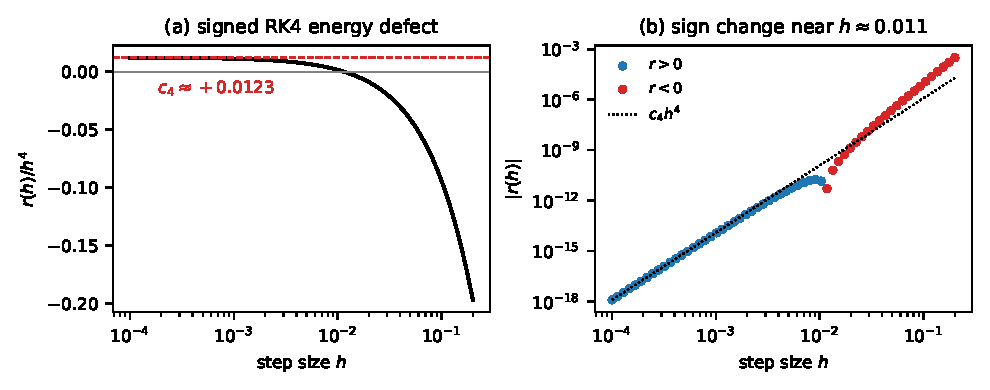
\includegraphics[width=0.95\linewidth]{fig/fig_sign.pdf}
\caption{RK4 energy defect at the start state, 40-digit arithmetic. (a)
$r/h^4$ crosses zero near $h\approx0.011$. (b) $|r|$ coloured by sign.}
\label{fig:sign}
\end{figure}

\end{document}
